\documentclass[hyperref={pdfpagelabels=false}]{beamer}
\graphicspath{{assets/}}
\usepackage{lmodern}
\usetheme{CambridgeUS}
\beamertemplatenavigationsymbolsempty


\renewcommand*{\bibfont}{\tiny}
 
\usepackage{media9}
\usepackage{booktabs}
\usepackage{graphics}
%% \usepackage{appendixnumberbeamer}
%% \expandafter\def\expandafter\insertshorttitle\expandafter{%
%%   \insertshorttitle\hfill\insertframenumber\,/\,\inserttotalframenumber}

\usepackage[backend=biber]{biblatex}
\addbibresource{assets/references.bib}

% Custom colors
% \usepackage{xcolor}
% http://www.computerhope.com/htmcolor.htm
% \definecolor{light blue}{HTML}{AAAAFF}
% \definecolor{light green}{HTML}{AAAAFF}

\makeatletter
\definecolor{mybackground}{HTML}{82CAFA}
\definecolor{myforeground}{HTML}{0000A0}

\setbeamertemplate{bibliography item}[text]

\setbeamercolor{normal text}{fg=black,bg=gray!10!white}
\setbeamercolor{alerted text}{fg=red}
\setbeamercolor{example text}{fg=black}

\setbeamercolor{background canvas}{fg=mybackground, bg=white}
\setbeamercolor{background}{fg=myforeground, bg=mybackground}

\setbeamercolor{palette primary}{fg=black, bg=blue!20!white}
\setbeamercolor{palette secondary}{fg=black, bg=blue!40!white}
\setbeamercolor{palette tertiary}{fg=black, bg=blue!60
  !white}
\setbeamercolor{frametitle}{fg=black, bg=gray!20!white}
\setbeamercolor{title}{fg=black, bg=gray!20!white}

\setbeamercolor{part title}{fg=black, bg=blue!60!white}
\makeatother


\usepackage{tkz-kiviat}
\usepackage{listings}

%% \documentclass[]{scrartcl}
%% \usepackage[utf8]{inputenc} 
%% \usepackage[T1]{fontenc}
%% \usepackage[upright]{fourier} 
%% \usepackage[usenames,dvipsnames]{xcolor}
%% \usepackage{tkz-kiviat,numprint,fullpage} 
%% \usetikzlibrary{arrows}
%% \thispagestyle{empty}


\definecolor{lightbg}{rgb}{0.9, 0.9, 0.95}
\definecolor{darkgreen}{rgb}{0, 0.7, 0}
\definecolor{brickred}{rgb}{0.8, 0.2, 0.2}
\definecolor{aquamarina}{rgb}{0, 0.7, 0.6}

\definecolor{visiblered}{rgb}{0.45, 0, 0}
\definecolor{visiblegreen}{rgb}{0, 0.4, 0}
\definecolor{visibleblue}{rgb}{0.1, 0.1, 0.45}






\title[Review of DL Frameworks]{A Review of Current Deep Learning Frameworks}  
\author[Andr\'es Fern\'andez Rodr\'iguez]{Andr\'es Fern\'andez Rodr\'iguez}
\institute[]{Software Engineering and Computer Vision}
\date{\today}%{October 13, 2017} 
\begin{document}
\titlegraphic{
\includegraphics[scale=0.15]{goethe-logo.png}}
     {\frame \titlepage}



     \begin{frame}
       \frametitle{Table of contents}
       \tableofcontents[hideallsubsections]
     \end{frame}




     %%%%%%%%%%%%%%%%%%%%%%%%%%%%%%%%%%%%%%%%%%%%%%%%%%%%%%%%%%%%%%%%%%%%%%%%%%%%%%%%%%%%%%%%
     \section{Approach}
     \frame{\sectionpage}
     %%%%%%%%%%%%%%%%%%%%%%%%%%%%%%%%%%%%%%%%%%%%%%%%%%%%%%%%%%%%%%%%%%%%%%%%%%%%%%%%%%%%%%%%

     \begin{frame}
       \frametitle{Goal and Structure}
       The goal of this review is to \textbf{provide information about current DL frameworks} together with \textbf{criteria to allow their comparison}. For that,
       \vspace{3mm}
       \begin{enumerate}[<.->]
       \item It will focus on several factors that I considered relevant for any framework, and for DL frameworks in particular. This is discussed in the present section, \textbf{approach}
       \item In the next section, several DL \textbf{frameworks} will be reviewed paying attention to the discussed factors
       \item Finally, all the given information will be collapsed to \textbf{sum-up} and allow comparisons among frameworks
       \item The information presented here comes \textbf{mostly from third-party sources}. Citations are marked in square brackets and attached in the \textbf{references} section
       \end{enumerate}

     \end{frame}

     %% \subsection{Definitions} %%%%%%%%%%%%%%%%%%%%%%%%%%%%%%%%%%%%%%%%%%%%%%%%%%%%%%%%%%%%%%%
     %% %% \frame{\subsectionpage}
     
     \begin{frame}
       \frametitle{Scope}
       The scope of this review are \textbf{current software frameworks that integrate many DL-related tasks}. In this context,

       \vspace{5mm}
       \begin{itemize}[<.->]
       \item \small{A \textbf{framework} is a consistent piece of software that provides solutions for domain-specific tasks, usually exposed through an extensible API}
       \item \small{A \textbf{DL}-related task is concerned with the design, implementation, training... of programs that perform deep learning, as well as the management of the data and hardware required for that task}
       \item \small{DL is a rapidly changing landscape, so \textbf{\textit{current}} doesn't necessarily mean \textit{new}: some frameworks have been there for a while and are still alive and kicking}
       \end{itemize}
     \end{frame}

     
      \begin{frame}
        \frametitle{Relevant Factors of a Framework: A Trade-Off}
        \begin{itemize}[<.->]
          \vspace{1mm}
       \item  \textbf{Resources required}
         \begin{itemize}[<.->]
         \item Money (fees, new hardware/software requirements, etc.)
         \item Time
           \begin{itemize}[<.->]
           \item Learning curve (structured API, long-lasting community)
           \item Runtime (at training and production stages)
           \item Development (verbosity, good documentation/help, IDE support)
           \item Non-Development (testing, debugging, visualizing...)
           \item Maintenance (stable API, large community)
           \end{itemize}
         \end{itemize}
         \vspace{4mm}
       \item \textbf{Value provided}
         \begin{itemize}[<.->]
         \item Fiability (numerical stability, big data+long duration)
         \item \textbf{API coverage and extendability (next slides)}
         \item Licensing
         \item Integration (saves time \& money)
           \begin{itemize}[<.->]
           \item With the language(s) (via libraries, CLI...)
           \item With communities (GitHub, model zoo, API stability...)
           \item With other frameworks (f.e. serialization via ONNX...)
           \item Further integration (O.S., PaaS, \{C$\mid$G$\mid$T$\mid$I\}PU...)
           \end{itemize}
         \end{itemize}
        \end{itemize}
        \vspace{4mm}
     \end{frame}


      \begin{frame}
        \frametitle{DL Frameworks: General Approach}

       \begin{block}{} % alertblock {Deep Learning...}
         \small{Deep Learning is an approach to AI that can safely be regarded as the study of models that involve a great amount of \textbf{composition of learned funcs.}\cite[p.8]{goodfellow}}
       \end{block}
       \vspace{2mm}

       \begin{columns}
         \column{0.5\linewidth}
         \centering
         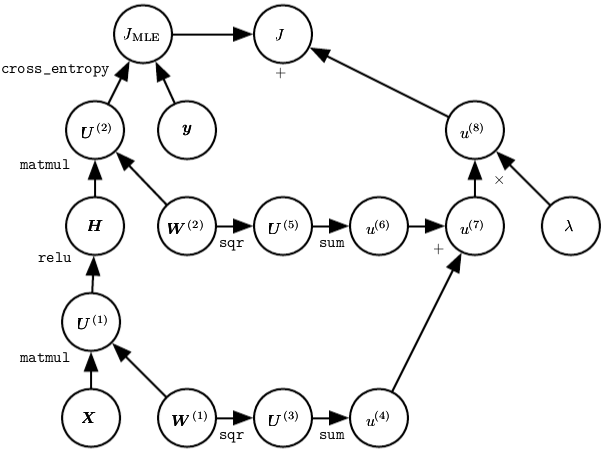
\includegraphics[scale=0.3]{mlp_graph_220.png}
         \column{0.49\linewidth}
         \centering
         \textbf{In DL Frameworks}:
         \begin{itemize}[<.->]
         \item \small{Computations organized in graphs}
         \item \small{Nodes$\Leftrightarrow$operations}
         \item \small{Inputs$\Leftrightarrow$leaves}
         \item \small{Every node can be an output}
         \item \small{Dataflow as tensors across nodes}
         \item \small{Different approaches for backprop.}
         \end{itemize}
       \end{columns}

       \begin{center}
         \\\scriptsize{From \cite[220]{goodfellow}: The computational graph corresponding to the following function composition:\\
           $J = \mathcal{L}(y,  relu(x^TW^{(1)})^TW^{(2)}) + \lambda \sum_{w_i \in(W^{(1)}, W^{(2)})} {w_i^2} $ } 
       \end{center}
     \end{frame}

      \begin{frame}
        \frametitle{DL Frameworks: API Coverage}
        The main actions to be done with this graphs are:
        \begin{itemize}[<.->]
       \item \small{Design and implement}
       \item \small{Train with backpropagation (+manage corresponding data and gradients)}
       \item \small{Deploy and run}
       \item \small{Test and debug}
       \item \small{Save, restore and serialize}
       \item \small{Visualize and/or communicate}
       \end{itemize}
        \vspace{2mm}
        For that, the APIs ideally provide:
       \begin{itemize}[<.->]
       \item \small{A comprehensive \textbf{Layer-API} with \textbf{differentiation} and batching}
       \item \small{A flexible \textbf{Model-API} supporting cyclic, dynamic graphs and param. sharing}
       \item \small{Facilities for \textbf{data} loading and management}
       \item \small{Facilities for testing, debugging and visualizing the graphs}
       \item \small{Support for (data/model) \textbf{parallelism} across different processing units}
       \item \small{Protocols for model \textbf{serialization} (architecture and parameters)}
       \item \small{Further desired features (DSP, PPLs...)}
       \end{itemize}
       \vspace{1mm}
       This can be achieved in different ways, as discussed in the following slides.
     \end{frame}


   
     %% \subsection{Criteria} %%%%%%%%%%%%%%%%%%%%%%%%%%%%%%%%%%%%%%%%%%%%%%%%%%
     %% %% \frame{\subsectionpage}

     
     \begin{frame}[fragile]
       \frametitle{Graph: Declarative vs. Imperative Design (by \cite[p.191]{petuum})}

       \noindent\begin{minipage}[t]{.55\textwidth}

       \textbf{Declarative}
       \begin{lstlisting}[
           numbers=left,
           numberstyle=\tiny,
           stepnumber=1,
           numbersep=5pt,
           frame=single,
           framerule=0pt,
           backgroundcolor=\color{lightbg},
           language=Python,
           basicstyle=\scriptsize,
           keywordstyle=\color{darkgreen},
           stringstyle=\color{brickred},
           commentstyle=\color{aquamarina}
         ]
A = Variable('A')
B = Variable('B')
C = B*A
# compiles the function
f = compile(C)
c = f(A=np.ones(10), B=np.ones(10)*2)
       \end{lstlisting}
       \end{minipage}\hfill
       \begin{minipage}[t]{.35\textwidth}

         \textbf{Imperative}
         \begin{lstlisting}[
             numbers=left,
             numberstyle=\tiny,
             stepnumber=1,
             numbersep=5pt,
             frame=single,
             framerule=0pt,
             backgroundcolor=\color{lightbg},
             language=Python,
             basicstyle=\scriptsize,
             keywordstyle=\color{darkgreen},
             stringstyle=\color{brickred},
             commentstyle=\color{aquamarina}]
import numpy as np
a = np.ones(10)
b = np.ones(10)*2
c = b*a
d = c+1
         \end{lstlisting}
       \end{minipage}


       \begin{columns}[t]
         \column{0.55\linewidth}
         \centering
         \begin{itemize}[<.->]
         \item \small{Static, \textit{whole-graph} model}
         \item \small{Easier to optimize (e.g. distributed, batching, parallelization, black magic...) for devs}
         \item \small{More efficient (deploy, train, run)}
         \end{itemize}
         
         \column{0.35\linewidth}
         \centering
         \begin{itemize}[<.->]
         \item \small{Dynamic, \textit{layer-by-layer} model}
         \item \small{More intuitive, less verbose}
         \item \small{More flexible (data and graph are on same level, see \texttt{*} op)}
         \item \small{Complex behind the scenes, less efficient}
         \end{itemize}
       \end{columns}
       
%% WARNING!! IN [fragile] SLIDES, THE \end{frame} STATEMENT HAS TO BE AT BEGINNING OF LINE AND HAVE NO COMMENTS AFTER (https://tex.stackexchange.com/a/277843)
\end{frame}


     \begin{frame}
       \frametitle{Graph: Dynamic Elements}
       \vspace{-2mm}
       Using a computational graph can present two types of dynamism:
       \begin{itemize}[<.->]
       \item \small{\textbf{Shape of data input/throughput} changes:\\
         With exceptions (like flattening or pyramidal pooling) static graphs adapt poorly to this type of dynamism}
       \item \small{\textbf{Connections} and \textbf{weights} change:}
         \begin{itemize}[<.->]
         \item \small{Variable connections aren't usually problematic if the elements are pre-compiled, and the framework allows for conditional flow}
         \item \small{Dynamic weight size is cumbersome even if the maximum can be allocated statically. Further solutions involve disabling the static graph checking (suboptimal)}
         \end{itemize}
       \end{itemize}
       \vspace{-3mm}
       \begin{center}
         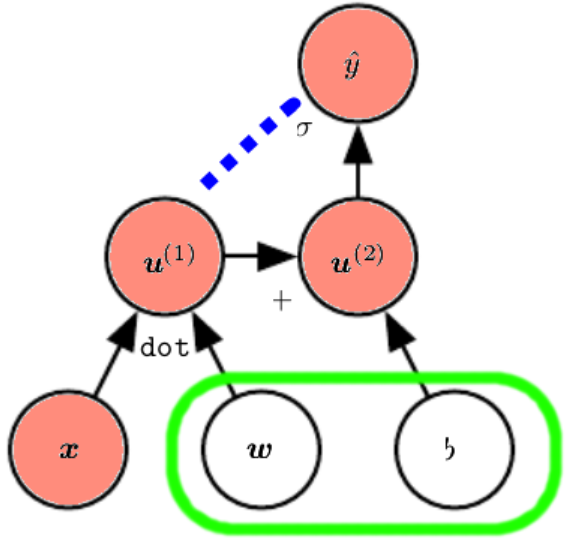
\includegraphics[scale=0.15]{logreg_graph_205.png}
         \scriptsize{\\For $\hat{y}=\sigma(x^Tw+b)$, basic example for dynamism in data (red), weights (green) and connections (blue). Adapted from \cite[p.205]{goodfellow}.}
       \end{center}
     \end{frame}

     \begin{frame}
       \frametitle{Graph: Gradient Calculation}
       \small{There are 3 popular methods to calculate the derivative, with diffent memory requirements, stability and performance features(\cite{bart-review}, \cite{dali-autodiff}, \cite{domluna-autodiff}, \cite{domke-autodiff})}:
       \begin{itemize}
       \item \scriptsize{\textbf{Numerical differentiation}: Imprecise, slow for high-dimensional data (used if $f$ unknown)}
       \item \scriptsize{\textbf{Symbolic differentiation}: Expression for every architecture not always easy/stable/optimal}
       \item \scriptsize{\textbf{Automatic differentiation (tape-based)}: Numerical+symbolic+chain rule (compromise)}
       \end{itemize}
       \vspace{-3mm}
       \begin{center}
         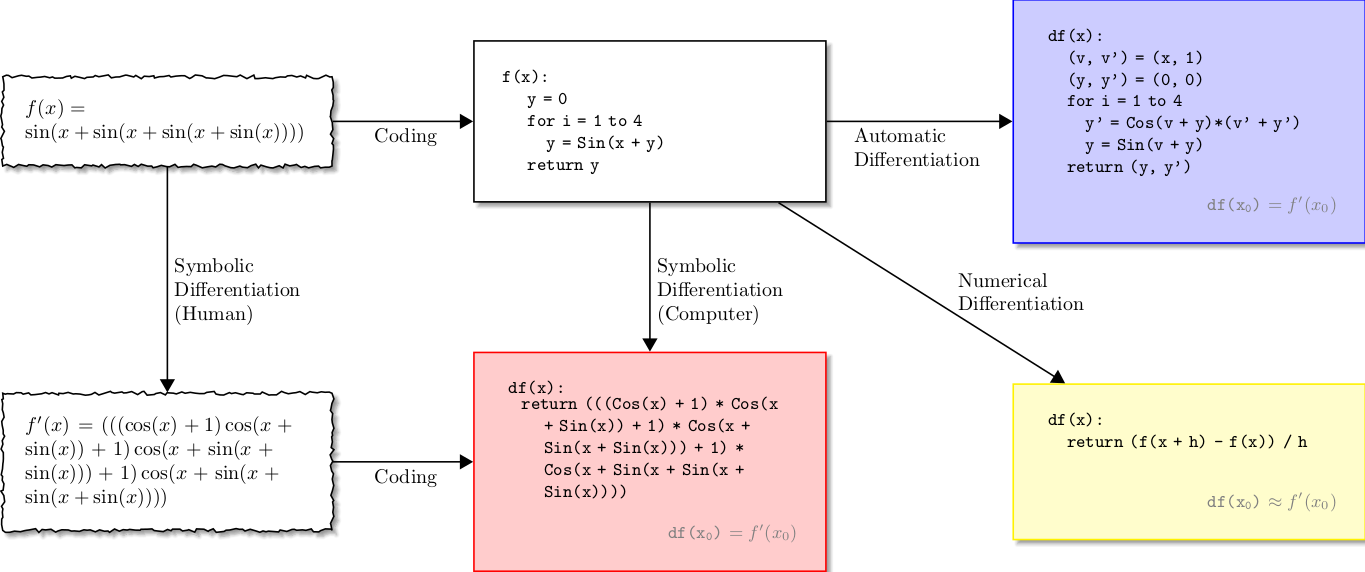
\includegraphics[scale=0.24]{autodiff_pic.png}
         \tiny{\\From \cite{autodiff-paper}: Differentiation of mathematical expressions and code. Symbolic differentiation (lower center); numerical differentiation (lower right); automatic differentiation (upper right)}
       \end{center}
     \end{frame}
     
     \begin{frame}
       \frametitle{Comparing Frameworks: Problematic}

       It is difficult to convey all the relevant factors of a DL framework in a compact, precise and unbiased way.\\[10pt]

       For instance, a Framework with a quick data loader and dynamic graph model may perform better or worse in runtime/training depending on the particularities of the graph, data and hardware involved.\\[10pt]

       There are even cases in which the development time is more important than the runtime and a smoother learning curve or specific languages are prioritized.\\[10pt]

       This review tries to achieve a compromise by combining 3 formats: \textbf{tabular}, \textbf{pros-cons} bullet list and \textbf{kiviat} diagram (discussed in the following slides).

     \end{frame}

     \begin{frame}
       \frametitle{Comparing Frameworks: Tabular Format}
       \vspace{6mm}
         \begin{columns}[t]
         \column{0.6\linewidth}
         \centering
         \small{Collapsed: info lost in specific/subjective goals}
         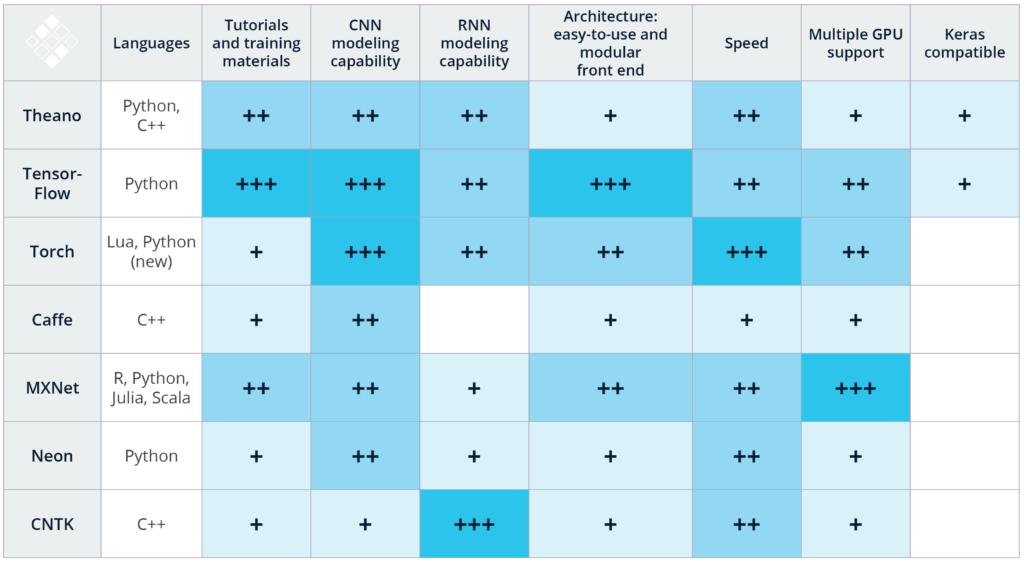
\includegraphics[scale=0.2]{comparison_svd.png}
         \\\scriptsize{From \cite{svd-review} (outdated): Has to be given along with the criteria to be interpretable}
         \column{0.4\linewidth}
         \centering
         \small{Extended: too sparse}
         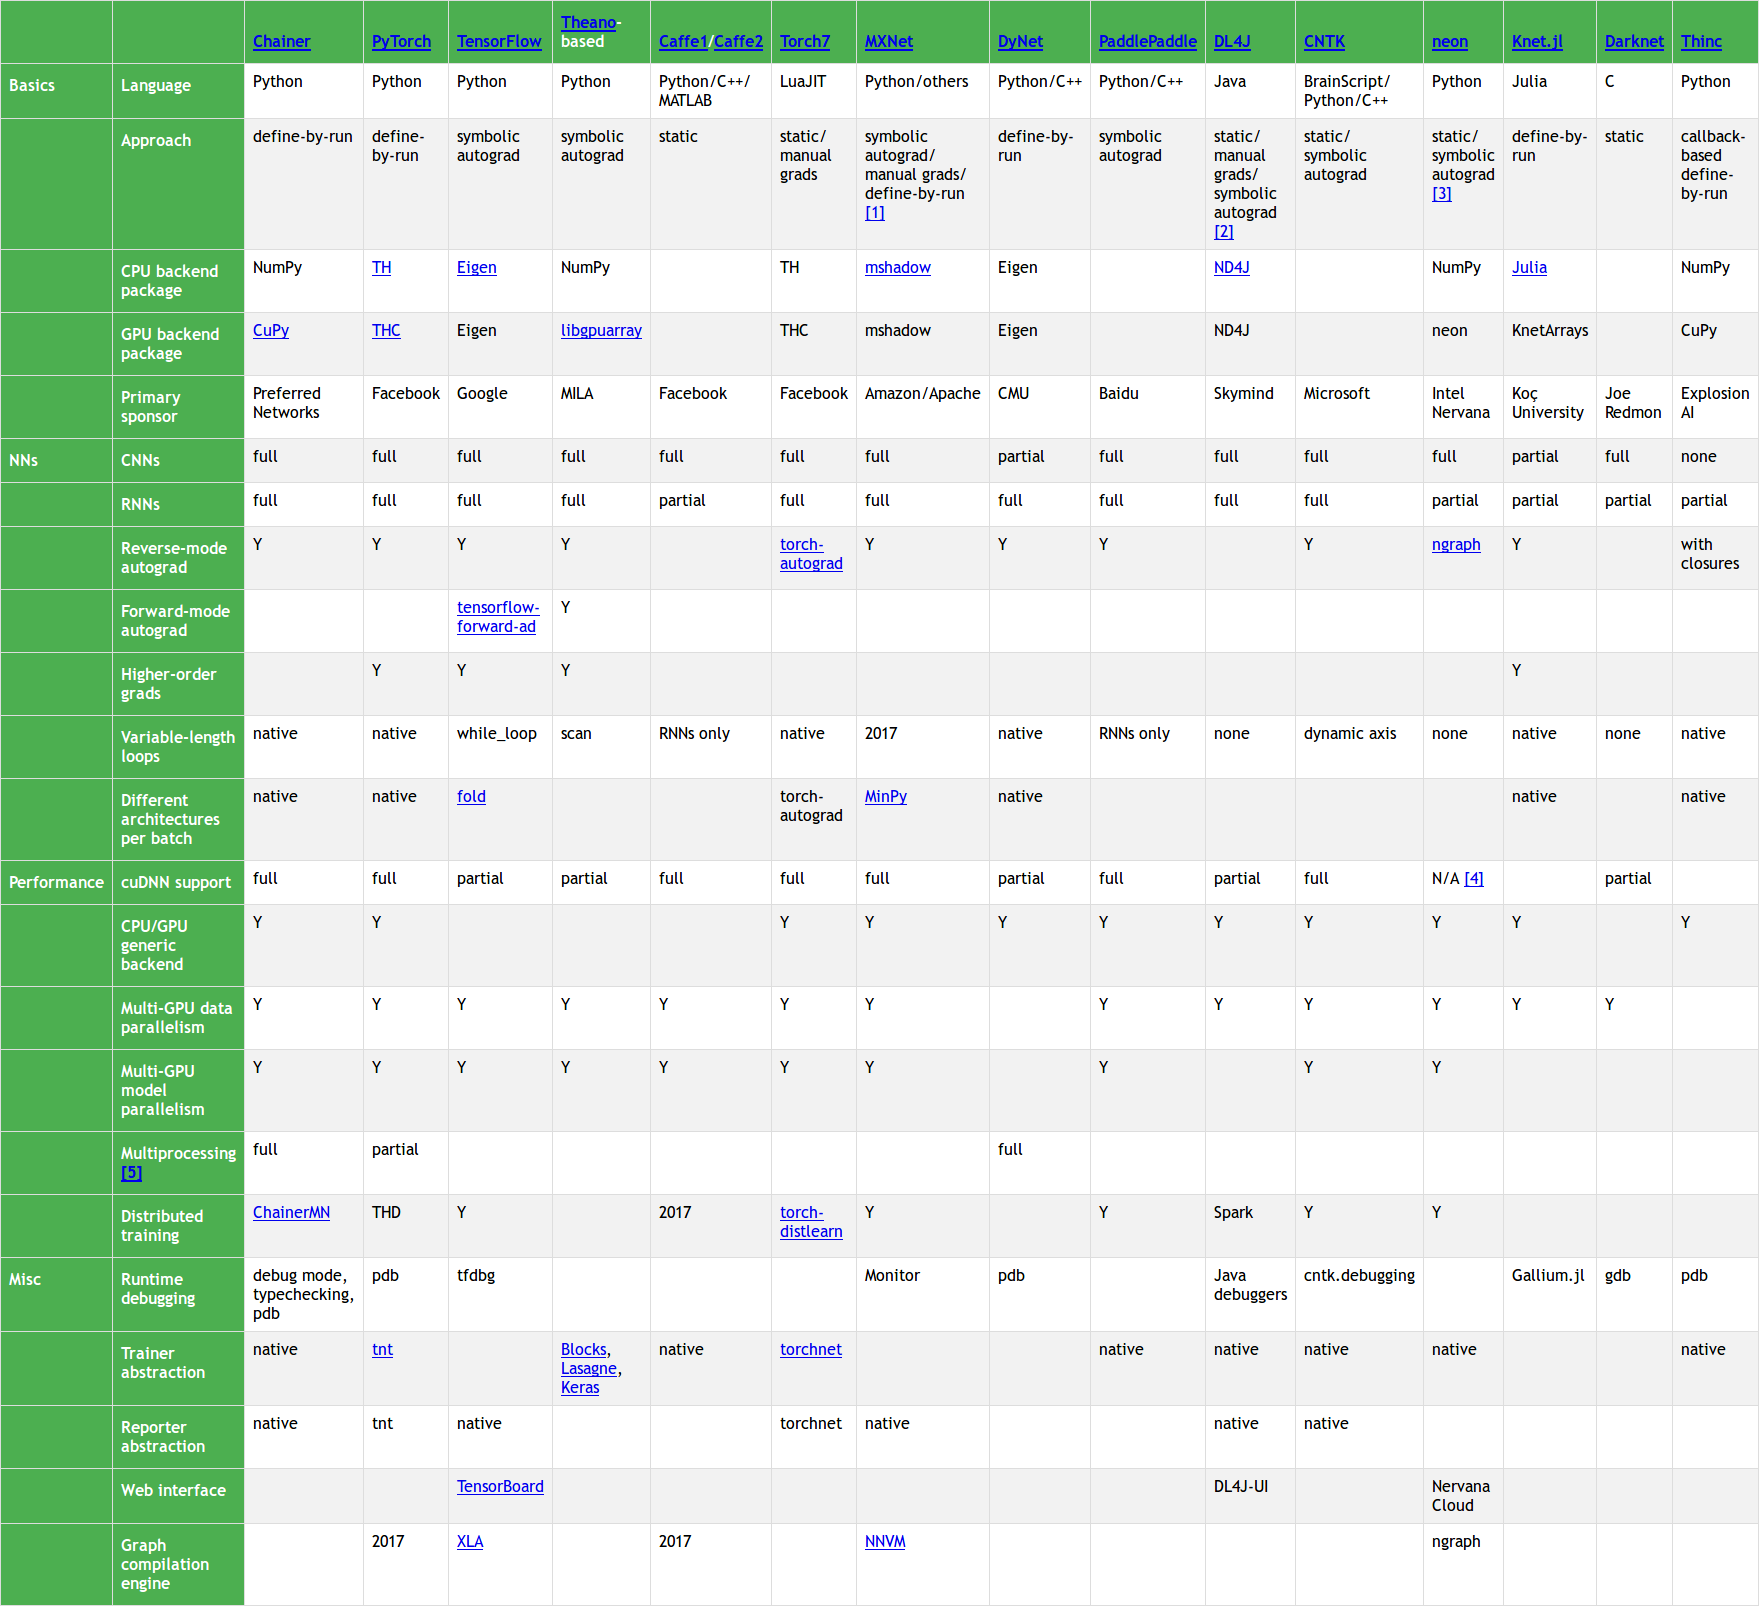
\includegraphics[scale=0.08]{comparison_chainer.png}
         \\\scriptsize{From \cite{chainer-review}: This table demands a significant amount of time to be fully explored}
         \end{columns}
         \vspace{6mm}
     \end{frame}

      \begin{frame}
        \frametitle{Comparing Frameworks: Pros-Cons Bullet List}
               \begin{itemize}
               \item[+]   \scriptsize{Qualitative and extended evaluation intuitively}
               \item[$-$] \scriptsize{Verbose, requires backing-up text}
               \item[$-$] \scriptsize{Less visual than extended tables and still sparse (inefficient for large number of factors)}
               \item[?] \scriptsize{Non normalized, allows for more freedom but structure becomes more arbitrary}
               \end{itemize}
               \vspace{0mm}
               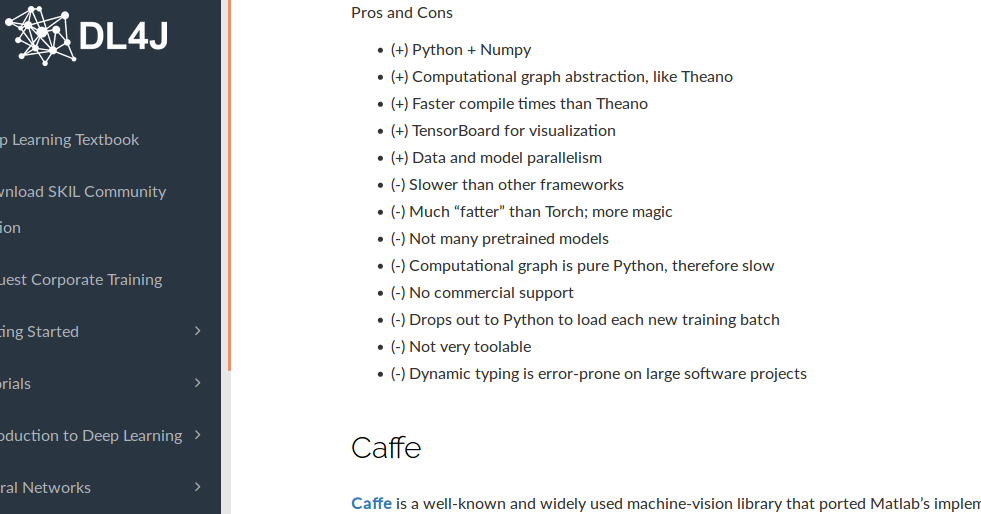
\includegraphics[scale=0.32]{pros_cons_list.png}
               \centering
               \\\tiny{From \cite{dl4j-review}: The DL4J webpage offers a review of several DL frameworks in this format}

               \vspace{6mm}
     \end{frame}

     \begin{frame}
       \frametitle{Comparing Frameworks: Kiviat Diagram - 1/2}
       \begin{itemize}
       \item[+]   \small{Compromise between qualitative and extended evaluation}
       \item[+]   \small{Very condensed: multiple elements (``rows'') per diagram possible}
       \item[$-$] \small{Bad handling of missing entries (zero-value? remove axis?)}
       \item[$-$] \small{Saturates if no. of axes and elements increase (can become ambiguous)}
       \end{itemize}
       \begin{columns}[t]
         \column{0.5\linewidth}
         \vspace{-9mm}
         \begin{tikzpicture}
           \tkzKiviatDiagram[scale=0.27,
             label space=9.5cm,
             radial  = 0,
             space=1,
             gap     = 1.17,
             lattice = 6]{
             \tiny{\textcolor{visiblered}{$\quad$1.platform/HW/\\[-6]$\quad$parall. support}},
             \tiny{\textcolor{visiblered}{\\[-1]2.run/train speed}},
             \tiny{\textcolor{visiblegreen}{\\[5]3.layer API}},
             \tiny{\textcolor{visiblegreen}{\\[5]4.model API}},
             \tiny{\textcolor{visiblegreen}{\\[-1]5.data tools}},
             \tiny{\textcolor{visiblegreen}{6.non-dev\\[-6]tools}},
             \tiny{\textcolor{visibleblue}{\\[5]7.documentation/\\[-6]learning curve}},
             \tiny{\textcolor{visibleblue}{\\[-8]8.Platforms/Languages/$\qquad\;$\\[-6] IDEs integration$\quad$}},
             \tiny{\textcolor{visibleblue}{\\[-8]$\qquad\qquad$9.HW/Parallelism\\[-6]$\qquad\qquad$transparency}},
             \tiny{\textcolor{visibleblue}{\\[2]10.healthy community/\\[-6] maintainability}}
           }
           \tkzKiviatLine[thick, % ultra thick
             color=green,
             % mark=none, % ball, mark size=5pt
             fill=green!10,
             opacity=1](4,5,5,3,6,2,4,5,4,4)
           \tkzKiviatLine[thick,
             color=blue,
             % fill=blue!10,
             opacity=0](4,3,5,3,3,6,4,3,3,5)
           \tkzKiviatLine[thick,
             color=red,
             % fill=red!10,
             opacity=0.5](4,5,5,5,4,6,4,3,2,3)

% \tkzKiviatGrad[unity=1](1)  
         \end{tikzpicture}
         
         \column{0.1\linewidth}
         
         \column{0.4\linewidth}
         \begin{itemize}[<.->]
         \item \scriptsize{Scores: 0 (center)$\Leftrightarrow$unknown, 1-6$\Leftrightarrow$worst to best}
         \item \scriptsize{Relevant factors collapsed into 11 axes, grouped as well in 3 colors: \textcolor{visiblered}{performance}, \textcolor{visiblegreen}{coverage}, \textcolor{visibleblue}{ecosystem}}
         \item \scriptsize{Compared elements can also have a color code to help interpretation (see example on the left: green element would be ambiguous without the filling)}
         \end{itemize}

       \end{columns}
     \end{frame}

    
     % fdsa

     % parallelism and HW transparency (batching, data, model)
     % integration to Platforms/languages/IDEs
     % HW support (especially multi-GPU)
     % run/train speed
     
     % debugging/testing/visualizing tools (Reporter?)
     % layer API + differentiation (higher-order grads?)
     % model building API (support CNN, RNN..., dynamism)
     % data management facilities
     
     % documentation+learning curve
     % healthy community (big/stable -> fiability)
     % maintainability (stable API, OSS, model serialization)
         
     % fee, licensing
     % languages supported
     % graph build paradigm
     % autodiff approach
     % host
     % further desired features (dsp, PPls)

\begin{frame}
  \frametitle{Comparing Frameworks: Kiviat Diagram - 2/2}
  \vspace{-2mm}
  \small{The \textcolor{visiblered}{performance} and \textcolor{visiblegreen}{coverage} axes follow these criteria}:
  \begin{itemize}
  \item \scriptsize{\textbf{Score=5}: The framework provides a competitive solution that adapts to the user's needs, via built-in functionality or flawless integration (matplotlib,  the Net class in PyTorch for NN design)}
  \item \scriptsize{\textbf{Score=4}: the framework provides a competitive but rigid/domain-specific solution (NN design in Caffe)}
  \item \scriptsize{\textbf{Score=3}: The framework provides convenient solution that is neither high-end nor easily customizable (TensorBoard)}
  \item \scriptsize{\textbf{Score=2}: the feature isn't provided by the framework, directly or via integration, and it has to (and \textit{can}) be manually developed}
  \item \scriptsize{\textbf{Score=1}: Inexistent/unfeasible solution}
  \end{itemize}
  \vspace{-1mm}
  \small{The \textcolor{visibleblue}{ecosystem} axes follow these criteria}:
  \begin{itemize}
  \item \scriptsize{\textbf{Score=5}: The framework is competitive with virtually no time overhead for the user}
  \item \scriptsize{\textbf{Score=4}: The user has to invest some time if no prior experience}
  \item \scriptsize{\textbf{Score=3}: The user has to invest time to get competitive}
  \item \scriptsize{\textbf{Score=2}: High time overhead, not competitive}
  \item \scriptsize{\textbf{Score=1}: Feature demands unfeasible amount of time}
  \end{itemize}
  \small{In all cases: \textbf{Score=0}: Not known, \textbf{Score=6} A speciality of the framework}
\end{frame}


\begin{frame}
       \frametitle{Example Combining Table, List and Kiviat: TensorFlow}
       \centering
       \renewcommand{\arraystretch}{0.8}
       \begin{tabular}{|c|c|}
         \hline
         \tiny{\textbf{Host} }   &  \tiny{Google, GitHub}\\
         \hline
         \tiny{\textbf{Fees, License} }   &  \tiny{No fees, Apache license since 2015\cite{tf-wiki})}\\
         \hline
         \tiny{\textbf{Graph Build} }   &  \tiny{Declarative}\\
         \hline
         \tiny{\textbf{Backprop. Model}    }   &  \tiny{Automatic differentiation}\\
         \hline
         \tiny{\textbf{Languages}\cite{tf-languages} }   &  \tiny{ \textcolor[rgb]{0,0.5,0}{C++, Python}, \textcolor[rgb]{0.8,0.8,0}{Java, Go, Ruby, R...\cite{r-tf-api}}}\\
         \hline
         \tiny{\textbf{Notes}}   &  \tiny{Successor of Theano, general purpose framework}\\
         \hline
       \end{tabular}
       \renewcommand{\arraystretch}{1}
          \begin{columns}[t]
         \column{0.5\linewidth}
         \vspace{-5mm}
         \begin{tikzpicture}
           \tkzKiviatDiagram[scale=0.27,
             label space=9.5cm,
             radial  = 0,
             space=1,
             gap     = 1.17,
             lattice = 6]{
             \tiny{\textcolor{visiblered}{$\quad$1.platform/HW/\\[-6]$\quad$parall. support}},
             \tiny{\textcolor{visiblered}{\\[-1]2.run/train speed}},
             \tiny{\textcolor{visiblegreen}{\\[5]3.layer API}},
             \tiny{\textcolor{visiblegreen}{\\[5]4.model API}},
             \tiny{\textcolor{visiblegreen}{\\[-1]5.data tools}},
             \tiny{\textcolor{visiblegreen}{6.non-dev\\[-6]tools}},
             \tiny{\textcolor{visibleblue}{\\[5]7.documentation/\\[-6]learning curve}},
             \tiny{\textcolor{visibleblue}{\\[-8]8.Platforms/Languages/$\qquad\;$\\[-6] IDEs integration$\quad$}},
             \tiny{\textcolor{visibleblue}{\\[-8]$\qquad\qquad$9.HW/Parallelism\\[-6]$\qquad\qquad$transparency}},
             \tiny{\textcolor{visibleblue}{\\[2]10.healthy community/\\[-6] maintainability}}
           }
           \tkzKiviatLine[ultra thick, % ultra thick
             color=black,
             % mark=none, % ball, mark size=5pt
             fill=orange!50,
             opacity=1](6,3,5,5,5,4,5,5,5,5)

% \tkzKiviatGrad[unity=1](1)  
         \end{tikzpicture}
         \column{0.08\linewidth}
         \column{0.42\linewidth}
         \begin{itemize}
         \item[\scriptsize{\textcolor{visiblered}{1.}}] \scriptsize{Runs on CPU, GPU, TPU, IPU, Android and embedded}
         \item[\scriptsize{\textcolor{visiblered}{2.}}] \scriptsize{\textbf{Dramatically} slower\cite{benchmark-paper17}\cite{u39kun-benchmark}\cite{chainer-benchmarks}}
         \item[\scriptsize{\textcolor{visiblegreen}{3.}}] \scriptsize{Very broad, $2^{nd}$-order derivatives}
         \item[\scriptsize{\textcolor{visiblegreen}{4.}}] \scriptsize{Data/parameter dynamism can be achieved with Eager\cite{tf-eager}}
         \item[\scriptsize{\textcolor{visiblegreen}{6.}}] \scriptsize{Provides all needed tools but require extra work (especially TensorBoard)}
         \item[\scriptsize{\textcolor{visibleblue}{8.}}] \scriptsize{Great support for C++/Python. Poor APIs+docs for the rest}
         \item[\scriptsize{\textcolor{visibleblue}{10.}}] \scriptsize{Broad and specialized community}
         \end{itemize}
       \end{columns}
     \end{frame}


\begin{frame}
  \frametitle{Approach: Summary}
  So far, the following has been discussed:
  \vspace{5mm}
  \begin{itemize}[<.->]
  \item The goals, structure and scope of this review\\[10pt]
  \item The desired features of a framework (general and DL-specific)\\[10pt]
  \item Some basic aspects of DL frameworks\\[10pt]
  \item Evaluation criteria and different representations to allow an effective comparison among frameworks
  \end{itemize}
  \vspace{5mm}
  The next section will discuss several frameworks, following this schema.
\end{frame}

     
     %%%%%%%%%%%%%%%%%%%%%%%%%%%%%%%%%%%%%%%%%%%%%%%%%%%%%%%%%%%%%%%%%%%%%%%%%%%%%%%%%%%%%%%%
     \section{Frameworks}
     \frame{\sectionpage}
     %%%%%%%%%%%%%%%%%%%%%%%%%%%%%%%%%%%%%%%%%%%%%%%%%%%%%%%%%%%%%%%%%%%%%%%%%%%%%%%%%%%%%%%%

     \subsection{Overview} %%%%%%%%%%%%%%%%%%%%%%%%%%%%%%%%%%%%%%%%%%%%%%%%%%%%%%%%
     %% \frame{\subsectionpage}
     \begin{frame}
       \frametitle{Some of the DL Frameworks Currently Avaliable}
       \begin{itemize}[<.->]

       \item  \textbf{Open-Source(d)}:
         \begin{itemize}[<.->]
         \item PyTorch (Facebook) $\leftarrow$ \textcolor{visiblered}{Torch (several)}
         \item Caffe2 (Facebook) $\leftarrow$ \textcolor{visiblered}{Caffe (BVLC)}
         \item TensorFlow (Google) $\leftarrow$ \textcolor{visiblered}{Theano (U. Montreal)}
         \item \small{MXNet (Apache)}
         \item \small{DL4J (Eclipse)}
         \item \small{CNTK (Microsoft)}
         \item \small{\textcolor{visiblered}{DyNet (Carnegie Mellon U.)}}
         \item \small{\textcolor{visiblered}{Chainer (U. Tokyo)}}
         \item \small{\textcolor{visiblered}{ConvNetJS (Karpathy)}}
         \item \small{POPLAR (GraphCore)}
         \item \small{And more (not covered): DIGITS (NVIDIA), Paddle (Baidu), Scikit-learn, SINGA and MLlib (Apache), neon (Intel)}
         \end{itemize}
       \end{itemize}
       \vspace{-2mm}

       \begin{minipage}[t]{0.45\textwidth}
         \vspace{0pt}
         \begin{itemize}[<.->]
           \item  \textbf{Closed-Source}:
             \begin{itemize}[<.->]
             \item \small{\textcolor{visiblered}{Mathematica (Wolfram)}}
             % \item \small{AML (Amazon)}
             \item \small{Michelangelo(Uber)}
             \end{itemize}
           \end{itemize}


       \end{minipage}%
       \hfill
       \begin{minipage}[t]{0.55\textwidth}
         \vspace{0pt}
         \begin{itemize}[<.->]
           \item  \textbf{Higher-Order}:
             \begin{itemize}[<.->]
             \item \small{\textcolor{visiblered}{Keras (on TF, Theano or CNTK)}}
             \item \small{\textcolor{visiblered}{Skorch (wraps PyTorch)}}
             \item \small{\textcolor{visiblered}{GLUON (on MXNet, CNTK)}}
             \end{itemize}
           \end{itemize}
       \end{minipage}
     \end{frame}


     %%    \begin{frame}
     %%      \frametitle{A first Sieve:}
     %%      Frameworks that have a small user/developer base for a long time are less likely to provide competitive featuers, and their fiability hasn't been proved through extensive use. This is the ``safer'' way of discarding them without looking into them (although it may be unfair). The following slides provide a current overview of their popularity.
     %% \end{frame}

    


     \begin{frame}
       \frametitle{Popularity at GitHub}
       \centering
       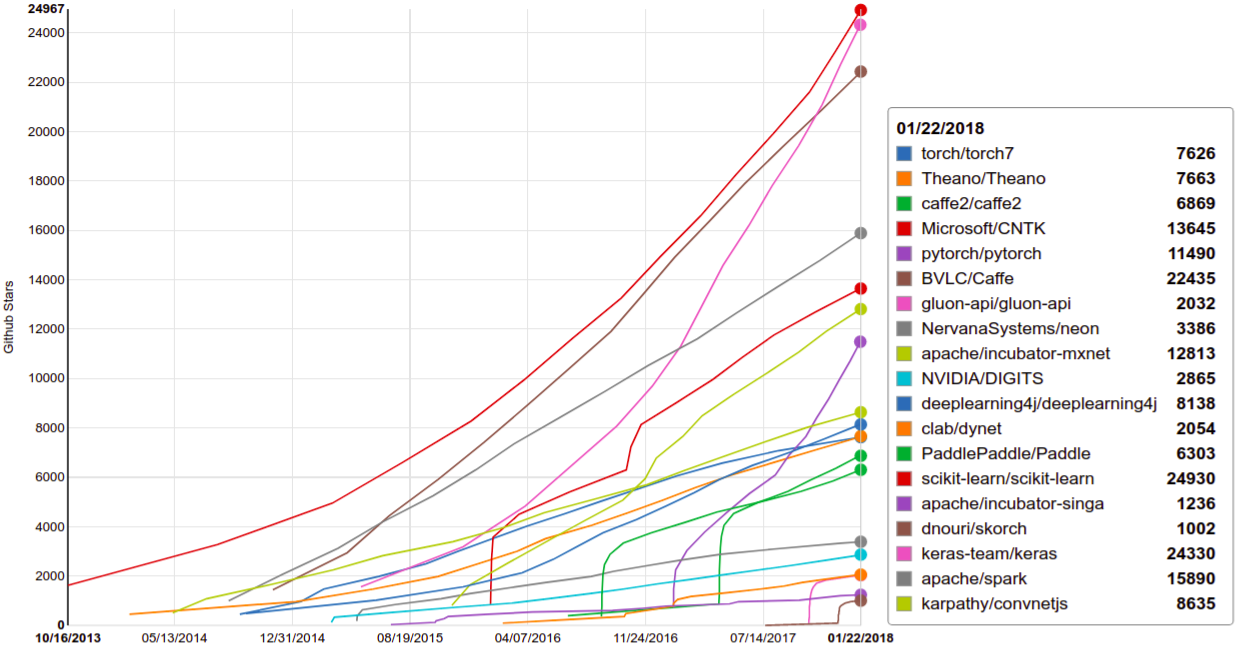
\includegraphics[scale=0.28]{github_stars_no_tf.png}
       \scriptsize{\\Repository stars on GitHub by date (generated with \cite{github-stars}). The TensorFlow repository, created at Nov.2015, has over 86k stars and was hidden for better visualization.}
     \end{frame}

      \begin{frame}
        \frametitle{Popularity at StackOverflow}
       % \textbf{Compact, fast to compute, continuous, meaningful, performative.}
       % \vspace{4mm}
       \begin{columns}
         \column{0.5\linewidth}
         \centering
         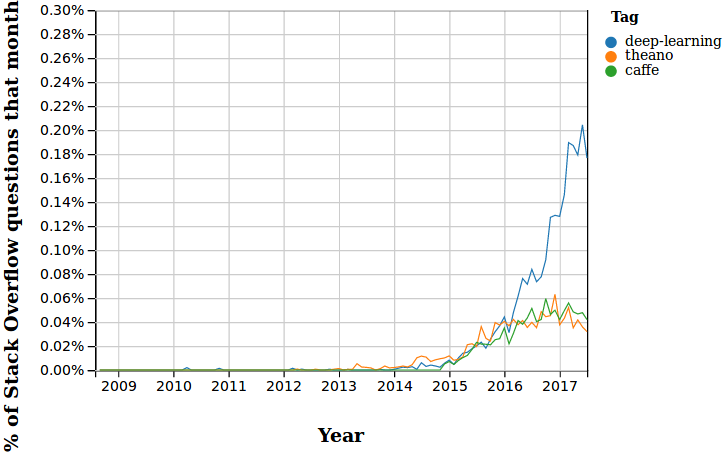
\includegraphics[scale=0.24]{SO_dl_theano_caffe.png}
         \column{0.5\linewidth}
         \centering
         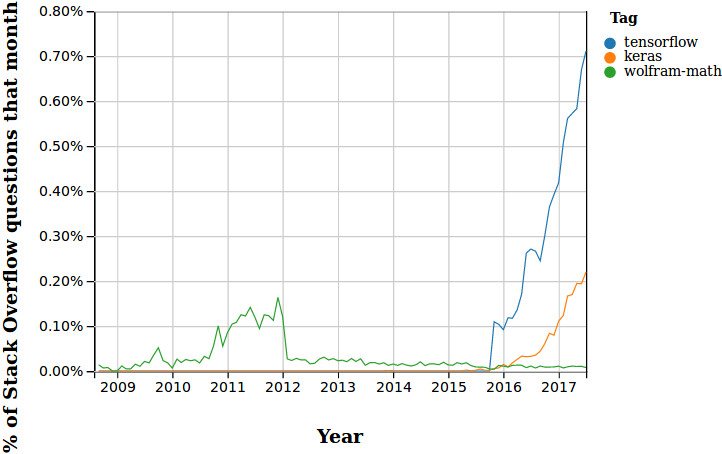
\includegraphics[scale=0.24]{SO_tf_keras_wolfram.png}
       \end{columns}
       \vspace{5mm}
       \centering
       \scriptsize{\\Popularity at StackOverflow for the existing tags\cite{so-trends}}
      \end{frame}

       \begin{frame}
       \frametitle{Popularity at ArXiv}
       % \textbf{Compact, fast to compute, continuous, meaningful, performative.}
       % \vspace{4mm}
       \centering
       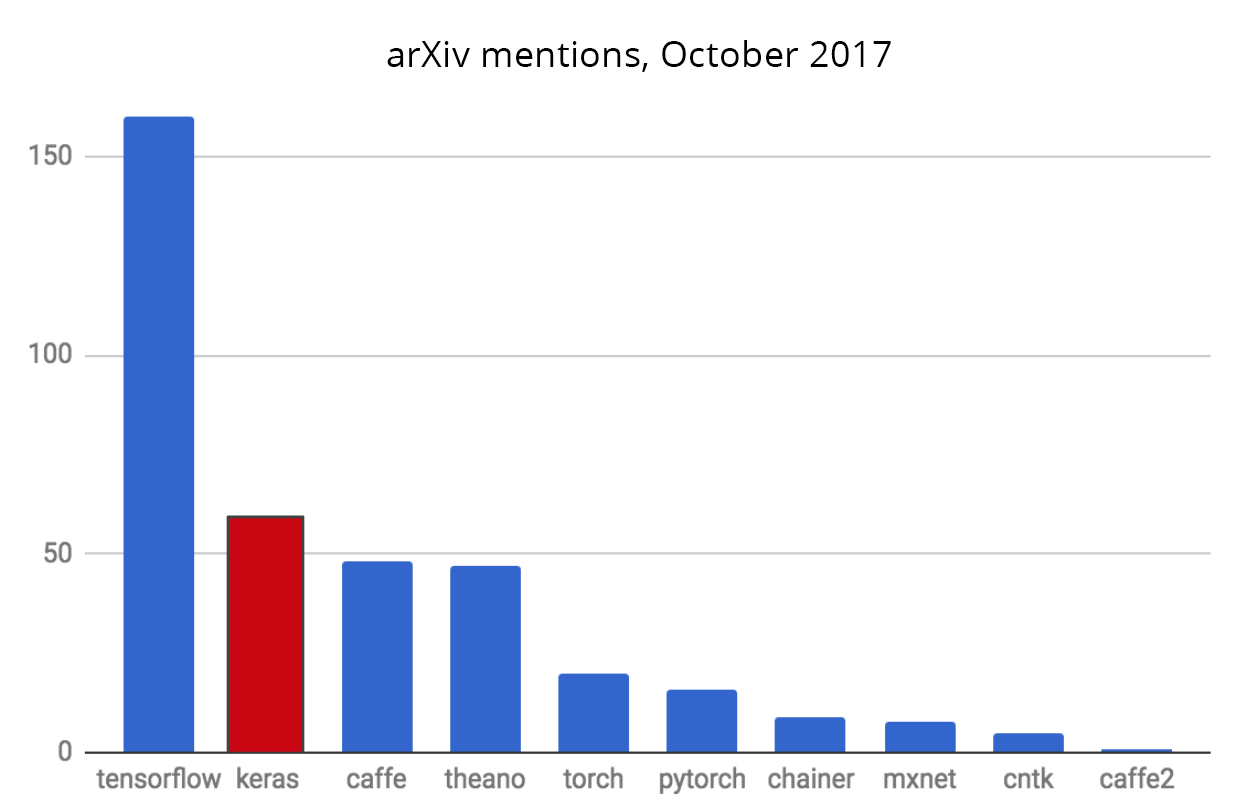
\includegraphics[scale=0.5]{arxiv_mentions.png}
       \scriptsize{\\Mentions in scientific papers uploaded to the preprint ArXiv.org server (from \cite{keras-web})}
     \end{frame}


     \subsection{TensorFlow} %%%%%%%%%%%%%%%%%%%%%%%%%%%%%%%%%%%%%%%%%%%%%%%%%%%%%%%%
     \begin{frame}[c] % [plain, c]
       \begin{center}
         \vspace{8mm}
         
\includegraphics[scale=0.15]{logo_tf.png}
       \end{center}
     \end{frame}

     \begin{frame}
       \frametitle{TensorFlow: Overview}
       \centering
       \renewcommand{\arraystretch}{0.8}
       \begin{tabular}{|c|c|}
         \hline
         \tiny{\textbf{Host} }   &  \tiny{Google, GitHub}\\
         \hline
         \tiny{\textbf{Fees, License} }   &  \tiny{No fees, Apache license since 2015\cite{tf-wiki})}\\
         \hline
         \tiny{\textbf{Graph Build} }   &  \tiny{Declarative}\\
         \hline
         \tiny{\textbf{Backprop. Model}    }   &  \tiny{Automatic differentiation}\\
         \hline
         \tiny{\textbf{Languages}\cite{tf-languages} }   &  \tiny{ \textcolor[rgb]{0,0.5,0}{C++, Python}, \textcolor[rgb]{0.8,0.8,0}{Java, Go, Ruby, R...\cite{r-tf-api}}}\\
         \hline
         \tiny{\textbf{Notes}}   &  \tiny{Successor of Theano, general purpose framework}\\
         \hline
       \end{tabular}
       \renewcommand{\arraystretch}{1}
          \begin{columns}[t]
         \column{0.5\linewidth}
         \vspace{-5mm}
         \begin{tikzpicture}
           \tkzKiviatDiagram[scale=0.27,
             label space=9.5cm,
             radial  = 0,
             space=1,
             gap     = 1.17,
             lattice = 6]{
  \tiny{\textcolor{visiblered}{$\quad$1.platform/HW/\\[-6]$\quad$parall. support}},
  \tiny{\textcolor{visiblered}{\\[-1]2.run/train speed}},
  \tiny{\textcolor{visiblegreen}{\\[5]3.layer API}},
  \tiny{\textcolor{visiblegreen}{\\[5]4.model API}},
  \tiny{\textcolor{visiblegreen}{\\[-1]5.data tools}},
  \tiny{\textcolor{visiblegreen}{6.non-dev\\[-6]tools}},
  \tiny{\textcolor{visibleblue}{\\[5]7.documentation/\\[-6]learning curve}},
  \tiny{\textcolor{visibleblue}{\\[-8]8.Platforms/Languages/$\qquad\;$\\[-6] IDEs integration$\quad$}},
  \tiny{\textcolor{visibleblue}{\\[-8]$\qquad\qquad$9.HW/Parallelism\\[-6]$\qquad\qquad$transparency}},
  \tiny{\textcolor{visibleblue}{\\[2]10.healthy community/\\[-6] maintainability}}
           }
           \tkzKiviatLine[ultra thick, % ultra thick
             color=black,
             % mark=none, % ball, mark size=5pt
             fill=orange!50,
             opacity=1](6,3,5,5,5,4,5,5,5,5)

% \tkzKiviatGrad[unity=1](1)  
         \end{tikzpicture}
         \column{0.08\linewidth}
         \column{0.42\linewidth}
         \begin{itemize}
         \item[\scriptsize{\textcolor{visiblered}{1.}}] \scriptsize{Runs on CPU, GPU, TPU, IPU, Android and embedded}
         \item[\scriptsize{\textcolor{visiblered}{2.}}] \scriptsize{\textbf{Dramatically} slower\cite{benchmark-paper17}\cite{u39kun-benchmark}\cite{chainer-benchmarks}}
         \item[\scriptsize{\textcolor{visiblegreen}{3.}}] \scriptsize{Very broad, $2^{nd}$-order derivatives}
         \item[\scriptsize{\textcolor{visiblegreen}{4.}}] \scriptsize{Data/parameter dynamism can be achieved with Eager\cite{tf-eager}}
         \item[\scriptsize{\textcolor{visiblegreen}{6.}}] \scriptsize{Provides all needed tools but require extra work (especially TensorBoard)}
         \item[\scriptsize{\textcolor{visibleblue}{8.}}] \scriptsize{Great support for C++/Python. Poor APIs+docs for the rest}
         \item[\scriptsize{\textcolor{visibleblue}{10.}}] \scriptsize{Broad and specialized community}
         \end{itemize}
          \end{columns}
     \end{frame}


     \begin{frame}
       \frametitle{TensorBoard: Problematic}
       \centering
       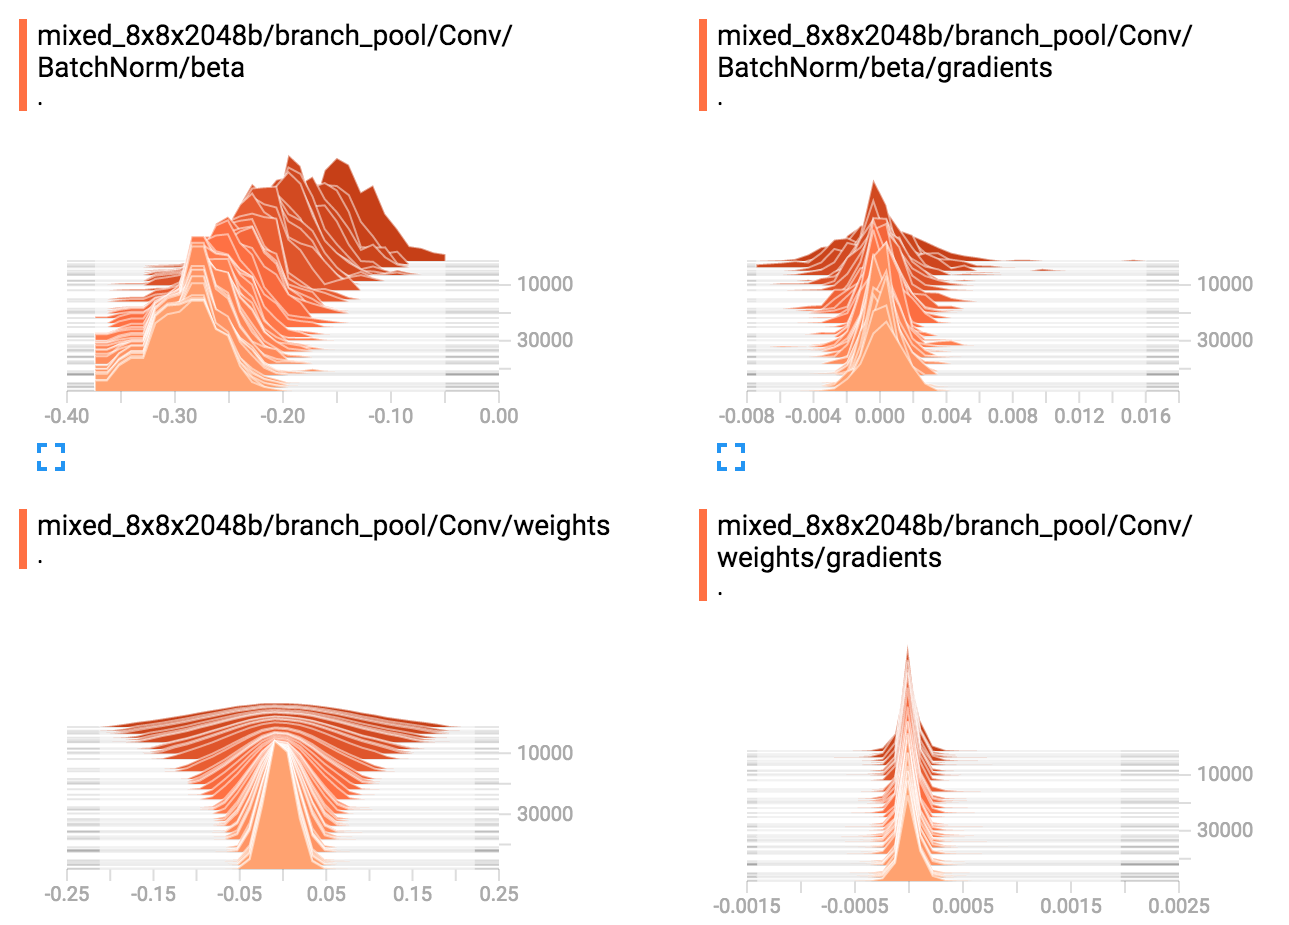
\includegraphics[scale=0.21]{tensorboard_hist.png}
       \scriptsize{\\TensorBoard is a very competent and convenient tool, but has its drawbacks. For example, the histograms are hardcoded to 30 bins, and the process of extending it is involved (photo: \cite{tb-photo}).}
     \end{frame}



     \subsection{PyTorch} %%%%%%%%%%%%%%%%%%%%%%%%%%%%%%%%%%%%%%%%%%%%%%%%%%%%%%%%
     \begin{frame}[c] % [plain, c]
       \begin{center}
         \vspace{8mm}
         %% \LARGE PyTorch\\
         %% \vspace{4mm}
         
\includegraphics[scale=0.15]{logo_pytorch.png}
       \end{center}
     \end{frame}


     \begin{frame}
       \frametitle{PyTorch: Overview}
       \centering
       \renewcommand{\arraystretch}{0.8}
       \begin{tabular}{|c|c|}
         \hline
         \tiny{\textbf{Host} }   &  \tiny{Facebook, GitHub}\\
         \hline
         \tiny{\textbf{Fees, License} }   &  \tiny{No fees, 3-Clause BSD since January, 2017\cite{dl4j-review}}\\
         \hline
         \tiny{\textbf{Graph Build} }   &  \tiny{Imperative (define-by-run)\cite{chainer-review}}\\
         \hline
         \tiny{\textbf{Backprop. Model}    }   &  \tiny{Automatic differentiation\cite{pytorch-web}}\\
         \hline
         \tiny{\textbf{Languages}\cite{tf-languages} }   &  \tiny{ \textcolor[rgb]{0,0.5,0}{Python}}\\
         \hline
         \tiny{\textbf{Notes}}   &  \tiny{Spin-off of Torch}\\
         \hline
       \end{tabular}
       \renewcommand{\arraystretch}{1}
          \begin{columns}[t]
         \column{0.5\linewidth}
         \vspace{-5mm}
         \begin{tikzpicture}
           \tkzKiviatDiagram[scale=0.27,
             label space=9.5cm,
             radial  = 0,
             space=1,
             gap     = 1.17,
             lattice = 6]{
  \tiny{\textcolor{visiblered}{$\quad$1.platform/HW/\\[-6]$\quad$parall. support}},
  \tiny{\textcolor{visiblered}{\\[-1]2.run/train speed}},
  \tiny{\textcolor{visiblegreen}{\\[5]3.layer API}},
  \tiny{\textcolor{visiblegreen}{\\[5]4.model API}},
  \tiny{\textcolor{visiblegreen}{\\[-1]5.data tools}},
  \tiny{\textcolor{visiblegreen}{6.non-dev\\[-6]tools}},
  \tiny{\textcolor{visibleblue}{\\[5]7.documentation/\\[-6]learning curve}},
  \tiny{\textcolor{visibleblue}{\\[-8]8.Platforms/Languages/$\qquad\;$\\[-6] IDEs integration$\quad$}},
  \tiny{\textcolor{visibleblue}{\\[-8]$\qquad\qquad$9.HW/Parallelism\\[-6]$\qquad\qquad$transparency}},
  \tiny{\textcolor{visibleblue}{\\[2]10.healthy community/\\[-6] maintainability}}
           }
           \tkzKiviatLine[ultra thick, % ultra thick
             color=black,
             % mark=none, % ball, mark size=5pt
             fill=violet!20,
             opacity=1](4,4,6,6,5,4,5,5,5,5)

% \tkzKiviatGrad[unity=1](1)  
         \end{tikzpicture}
         \column{0.08\linewidth}
         \column{0.42\linewidth}
         \begin{itemize}
         \item[\scriptsize{\textcolor{visiblered}{1.}}] \scriptsize{``essentially a GPU NumPy replacement''\cite{pytorch-vs-tf} + autograd}
         \item[\scriptsize{\textcolor{visiblegreen}{2.}}] \scriptsize{Extremely dynamic graph lifecycle may slow down some setups}
         \item[\scriptsize{\textcolor{visiblegreen}{4.}}] \scriptsize{PyTorch is especially capable for trying out new models}
         \item[\scriptsize{\textcolor{visiblegreen}{6.}}] \scriptsize{Relying highly in Python, requires some extra work for DL-specific (especially TensorBoard)}
         \item[\scriptsize{\textcolor{visibleblue}{8.}}] \scriptsize{Arguably Python is all you need}
         \item[\scriptsize{\textcolor{visibleblue}{9.}}] \scriptsize{Almost zero code overhead between CPU and GPU model}
         \item[\scriptsize{\textcolor{visibleblue}{10.}}] \scriptsize{Fastest growing + ONNX}
         \end{itemize}
          \end{columns}
          
     \end{frame}



     \begin{frame}
       \frametitle{About Open Neural Network Exchange (ONNX)}
       Specification for serializing trained models (similar to Google's \textbf{protobuf})
       \begin{itemize}[<.->]
       \item{Effort by Microsoft and Facebook (Amazon joined) to bridge the gap between model development and production. MIT License}
       \item{Released on September 2017, supported by CNTK, PyTorch, Caffe2, MXNet and Nvidia's TensorRT}
       \item{For static graph definitions, it only requires translation}
       \item {Branching only partially allowed (for shape operations etc): dynamic flow control not supported}
       \item {Graph visualization tools: NetDrawer (see picture from \cite{onnx-repo}) and Netron (interactive, supports also TF/Keras)}
       \end{itemize}
       
       \centering
       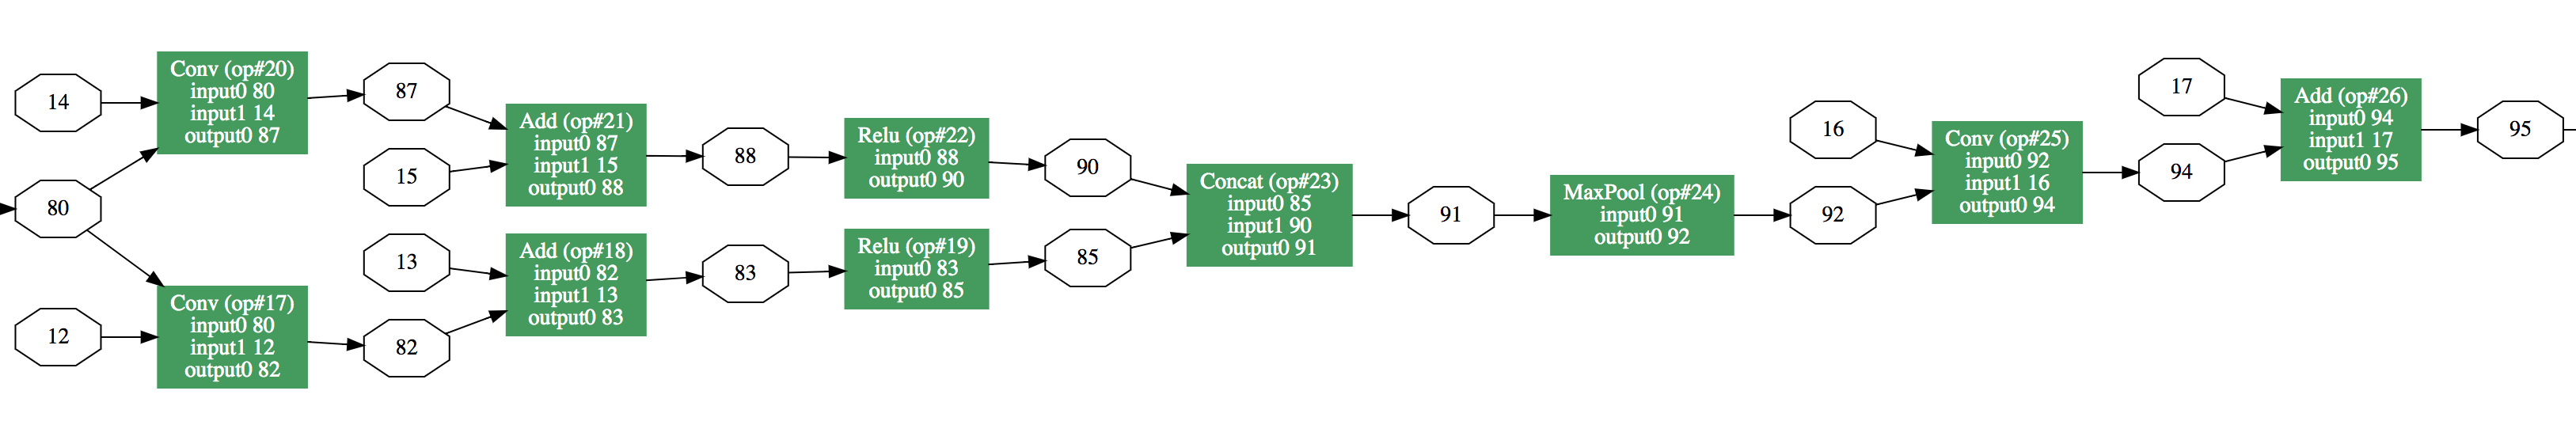
\includegraphics[scale=0.2]{onnx_visualization.png}
       % \scriptsize{\\ (from \cite{onnx-repo}).}
     \end{frame}


     \subsection{Caffe2} %%%%%%%%%%%%%%%%%%%%%%%%%%%%%%%%%%%%%%%%%%%%%%%%%%%%%%%%
     \begin{frame}[c] % [plain, c]
       \begin{center}
         \vspace{8mm}
         
\includegraphics[scale=0.2]{logo_caffe2.png}
       \end{center}
     \end{frame}

     \begin{frame}
       \frametitle{Caffe2: Overview}
       \centering
       \renewcommand{\arraystretch}{0.8}
       \begin{tabular}{|c|c|}
         \hline
         \tiny{\textbf{Host} }   &  \tiny{Facebook, GitHub}\\
         \hline
         \tiny{\textbf{Fees, License} }   &  \tiny{No fees, Apache2.0 license since April 2017)}\\
         \hline
         \tiny{\textbf{Graph Build} }   &  \tiny{Static (plaintext schemas)\cite{caffe2-web}}\\
         \hline
         \tiny{\textbf{Backprop. Model}    }   &  \tiny{Automatic differentiation\cite{caffe2-web}}\\
         \hline
         \tiny{\textbf{Languages}\cite{tf-languages} }   &  \tiny{ \textcolor[rgb]{0,0.5,0}{C++, Python}}\\
         \hline
         \tiny{\textbf{Notes}}   &  \tiny{Successor of Caffe, focus on modularity and scalability\cite{about-caffe2-birth}. Unlike Caffe, not only vision}\\
         \hline
       \end{tabular}
       \renewcommand{\arraystretch}{1}
          \begin{columns}[t]
         \column{0.5\linewidth}
         \vspace{-5mm}
         \begin{tikzpicture}
           \tkzKiviatDiagram[scale=0.27,
             label space=9.5cm,
             radial  = 0,
             space=1,
             gap     = 1.17,
             lattice = 6]{
  \tiny{\textcolor{visiblered}{$\quad$1.platform/HW/\\[-6]$\quad$parall. support}},
  \tiny{\textcolor{visiblered}{\\[-1]2.run/train speed}},
  \tiny{\textcolor{visiblegreen}{\\[5]3.layer API}},
  \tiny{\textcolor{visiblegreen}{\\[5]4.model API}},
  \tiny{\textcolor{visiblegreen}{\\[-1]5.data tools}},
  \tiny{\textcolor{visiblegreen}{6.non-dev\\[-6]tools}},
  \tiny{\textcolor{visibleblue}{\\[5]7.documentation/\\[-6]learning curve}},
  \tiny{\textcolor{visibleblue}{\\[-8]8.Platforms/Languages/$\qquad\;$\\[-6] IDEs integration$\quad$}},
  \tiny{\textcolor{visibleblue}{\\[-8]$\qquad\qquad$9.HW/Parallelism\\[-6]$\qquad\qquad$transparency}},
  \tiny{\textcolor{visibleblue}{\\[2]10.healthy community/\\[-6] maintainability}}
           }
           \tkzKiviatLine[ultra thick, % ultra thick
             color=black,
             % mark=none, % ball, mark size=5pt
             fill=grey!50,
             opacity=1](5,6,5,4,5,3,3,5,5,5)

% \tkzKiviatGrad[unity=1](1)  
         \end{tikzpicture}
         \column{0.08\linewidth}
         \column{0.42\linewidth}
         \begin{itemize}
         \item[\scriptsize{\textcolor{visiblered}{1.}}] \scriptsize{CPU, GPU, Android and iOS}
         \item[\scriptsize{\textcolor{visiblegreen}{3.}}] \scriptsize{Very rich and extendible DL API}
         \item[\scriptsize{\textcolor{visiblegreen}{4.}}] \scriptsize{Static model performs but prevents dynamism}
         \item[\scriptsize{\textcolor{visiblegreen}{6.}}] \scriptsize{Provides all needed tools but requires extra work (many dependencies)}
         \item[\scriptsize{\textcolor{visibleblue}{7.}}] \scriptsize{well structured docs but lacking}
         \item[\scriptsize{\textcolor{visibleblue}{8.}}] \scriptsize{Great support for C++/Python. Poor APIs+docs for the rest}
         \item[\scriptsize{\textcolor{visibleblue}{9.}}] \scriptsize{Flawless transparency}
         \item[\scriptsize{\textcolor{visibleblue}{10.}}] \scriptsize{As in Caffe, outstanding model zoo+incoming ONNX\cite{onnx}}
         \end{itemize}
          \end{columns}
     \end{frame}


      \begin{frame}
       \frametitle{From Caffe to caffe2: Example}
       Purposes in the origins of caffe2\cite{about-caffe2-birth}:
       \begin{itemize}[<.->]
       \item Faster experimenting and prototyping (see picture)
       \item Simpler compilation (restructuring dependencies)
       \item More portability (CPU/CUDA, Android, further)
       \end{itemize}
       \vspace{4mm}
       \begin{center}
         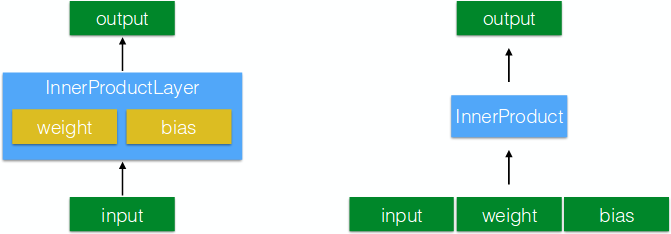
\includegraphics[scale=0.46]{improve_caffe.png}
         \scriptsize{\\Difference in design: from Caffe's \textit{Layers} (left) to Caffe2's \textit{Operators} (right)\cite{improving-caffe}}
       \end{center}
       \end{frame}

      




     \subsection{CNTK} %%%%%%%%%%%%%%%%%%%%%%%%%%%%%%%%%%%%%%%%%%%%%%%%%%%%%%%%
     \begin{frame}[c] % [plain, c]
       \begin{center}
         \vspace{8mm}
         
\includegraphics[scale=0.2]{logo_cntk.png}
       \end{center}
     \end{frame}

     \begin{frame}
       \frametitle{Cognitive Toolkit (CNTK): Overview}
       \centering
       \renewcommand{\arraystretch}{0.8}
       \begin{tabular}{|c|c|}
         \hline
         \tiny{\textbf{Host} }   &  \tiny{Microsoft, GitHub}\\
         \hline
         \tiny{\textbf{Fees, License} }   &  \tiny{No fees, almost-OS license\cite{dl4j-review} since Jan 2016)}\\
         \hline
         \tiny{\textbf{Graph Build} }   &  \tiny{Declarative\cite{cntk-web}}\\
         \hline
         \tiny{\textbf{Backprop. Model}    }   &  \tiny{Automatic differentiation\cite{cntk-web}}\\
         \hline
         \tiny{\textbf{Languages}\cite{cntk-web} }   &  \tiny{ \textcolor[rgb]{0,0.5,0}{C++, C\#, Python, BrainScript}, \textcolor[rgb]{0.8,0.8,0}{Java}}\\
         \hline
         \tiny{\textbf{Notes}}   &  \tiny{Apparently what MS internally uses\cite{cntk-reasons}}\\
         \hline
       \end{tabular}
       \renewcommand{\arraystretch}{1}
          \begin{columns}[t]
         \column{0.5\linewidth}
         \vspace{-5mm}
         \begin{tikzpicture}
           \tkzKiviatDiagram[scale=0.27,
             label space=9.5cm,
             radial  = 0,
             space=1,
             gap     = 1.17,
             lattice = 6]{
  \tiny{\textcolor{visiblered}{$\quad$1.platform/HW/\\[-6]$\quad$parall. support}},
  \tiny{\textcolor{visiblered}{\\[-1]2.run/train speed}},
  \tiny{\textcolor{visiblegreen}{\\[5]3.layer API}},
  \tiny{\textcolor{visiblegreen}{\\[5]4.model API}},
  \tiny{\textcolor{visiblegreen}{\\[-1]5.data tools}},
  \tiny{\textcolor{visiblegreen}{6.non-dev\\[-6]tools}},
  \tiny{\textcolor{visibleblue}{\\[5]7.documentation/\\[-6]learning curve}},
  \tiny{\textcolor{visibleblue}{\\[-8]8.Platforms/Languages/$\qquad\;$\\[-6] IDEs integration$\quad$}},
  \tiny{\textcolor{visibleblue}{\\[-8]$\qquad\qquad$9.HW/Parallelism\\[-6]$\qquad\qquad$transparency}},
  \tiny{\textcolor{visibleblue}{\\[2]10.healthy community/\\[-6] maintainability}}
           }
           \tkzKiviatLine[ultra thick, % ultra thick
             color=black,
             % mark=none, % ball, mark size=5pt
             fill=green!30,
             opacity=1](3,5,5,5,4,5,5,6,5,3)

% \tkzKiviatGrad[unity=1](1)  
         \end{tikzpicture}
         \column{0.08\linewidth}
         \column{0.42\linewidth}
         \begin{itemize}
         \item[\scriptsize{\textcolor{visiblered}{1.}}] \scriptsize{High-scale CPU/GPU, no traces of anything else}
         \item[\scriptsize{\textcolor{visiblered}{2.}}] \scriptsize{Much faster than TF (\cite{chainer-benchmarks})}
         \item[\scriptsize{\textcolor{visiblegreen}{3.}}] \scriptsize{Claimed very broad\cite{cntk-web}}
         \item[\scriptsize{\textcolor{visiblegreen}{4.}}] \scriptsize{Very comprehensive support (also through higher-order APIs)}
         \item[\scriptsize{\textcolor{visiblegreen}{6.}}] \scriptsize{Indirect support but very well documented}
         \item[\scriptsize{\textcolor{visibleblue}{8.}}] \scriptsize{One of the greatest strengths}
         \item[\scriptsize{\textcolor{visibleblue}{10.}}] \scriptsize{Small user base, restrictive licensing. But connections to Keras, Gluon, ONNX}
         \end{itemize}
          \end{columns}
     \end{frame}


     \subsection{DL4J} %%%%%%%%%%%%%%%%%%%%%%%%%%%%%%%%%%%%%%%%%%%%%%%%%%%%%%%%
     \begin{frame}[c] % [plain, c]
       \begin{center}
         \vspace{8mm}
         
\includegraphics[scale=0.17]{logo_dl4j.png}
       \end{center}
     \end{frame}
     
     
     \begin{frame}
       \frametitle{Deep Learning for Java (DL4J): Overview}
       \centering
       \renewcommand{\arraystretch}{0.8}
       \begin{tabular}{|c|c|}
         \hline
         \tiny{\textbf{Host} }   &  \tiny{Eclipse, GitHub}\\
         \hline
         \tiny{\textbf{Fees, License} }   &  \tiny{No fees, Apache2.0 license\cite{dl4j-repo}, release 0.92 in Dec 2017}\\
         \hline
         \tiny{\textbf{Graph Build} }   &  \tiny{Declarative\cite{dl4j-web}}\\
         \hline
         \tiny{\textbf{Backprop. Model}    }   &  \tiny{NOT AD (but unclear what, see \cite{dl4j-devguide})}\\
         \hline
         \tiny{\textbf{Languages}\cite{dl4j-repo} }   &  \tiny{\textcolor[rgb]{0,0.5,0}{Java, Scala}}\\
         \hline
         \tiny{\textbf{Notes}}   &  \tiny{CoC on the JVM, emphasis on scalability, UI and data management}\\
         \hline
       \end{tabular}
       \renewcommand{\arraystretch}{1}
          \begin{columns}[t]
         \column{0.5\linewidth}
         \vspace{-5mm}
         \begin{tikzpicture}
           \tkzKiviatDiagram[scale=0.27,
             label space=9.5cm,
             radial  = 0,
             space=1,
             gap     = 1.17,
             lattice = 6]{
  \tiny{\textcolor{visiblered}{$\quad$1.platform/HW/\\[-6]$\quad$parall. support}},
  \tiny{\textcolor{visiblered}{\\[-1]2.run/train speed}},
  \tiny{\textcolor{visiblegreen}{\\[5]3.layer API}},
  \tiny{\textcolor{visiblegreen}{\\[5]4.model API}},
  \tiny{\textcolor{visiblegreen}{\\[-1]5.data tools}},
  \tiny{\textcolor{visiblegreen}{6.non-dev\\[-6]tools}},
  \tiny{\textcolor{visibleblue}{\\[5]7.documentation/\\[-6]learning curve}},
  \tiny{\textcolor{visibleblue}{\\[-8]8.Platforms/Languages/$\qquad\;$\\[-6] IDEs integration$\quad$}},
  \tiny{\textcolor{visibleblue}{\\[-8]$\qquad\qquad$9.HW/Parallelism\\[-6]$\qquad\qquad$transparency}},
  \tiny{\textcolor{visibleblue}{\\[2]10.healthy community/\\[-6] maintainability}}
           }
           \tkzKiviatLine[ultra thick, % ultra thick
             color=black,
             % mark=none, % ball, mark size=5pt
             fill=visibleblue!70,
             opacity=1](5,5,4,4,6,5,5,5,5,5)

% \tkzKiviatGrad[unity=1](1)  
         \end{tikzpicture}
         \column{0.08\linewidth}
         \column{0.42\linewidth}
         \begin{itemize}
         \item[\scriptsize{\textcolor{visiblered}{1.}}] \scriptsize{JVM(CPU/GPU/Android) with Spark, Hadoop, Kafka}
         \item[\scriptsize{\textcolor{visiblered}{2.}}] \scriptsize{Speed=Caffe, $>$ TF/Torch (measuring data loading)\cite{dl4j-review}}
         \item[\scriptsize{\textcolor{visiblegreen}{3.}}] \scriptsize{No AD, cumbersome to extend}
         \item[\scriptsize{\textcolor{visiblegreen}{3.}}] \scriptsize{Lacking GANs, some RNNs...}
         \item[\scriptsize{\textcolor{visiblegreen}{5.,6.}}] \scriptsize{Outstanding. The speciality of DL4J}
         \item[\scriptsize{\textcolor{visibleblue}{8.}}] \scriptsize{Arguably Java is all you need}
         \item[\scriptsize{\textcolor{visibleblue}{10.}}] \scriptsize{Less structured than other frameworks\cite{dl4j-devguide}. One of the few providing corporate support. Model Zoo + Keras frontend}
         \end{itemize}
          \end{columns}
     \end{frame}


     

     \subsection{MXNet} %%%%%%%%%%%%%%%%%%%%%%%%%%%%%%%%%%%%%%%%%%%%%%%%%%%%%%%%
     \begin{frame}[c] % [plain, c]
       \begin{center}
         \vspace{8mm}
         
\includegraphics[scale=0.14]{logo_mxnet.png}
       \end{center}
     \end{frame}


     \begin{frame}
       \frametitle{MXNet: Overview}
       \centering
       \renewcommand{\arraystretch}{0.8}
       \begin{tabular}{|c|c|}
         \hline
         \tiny{\textbf{Host} }   &  \tiny{Apache, Amazon, GitHub}\\
         \hline
         \tiny{\textbf{Fees, License} }   &  \tiny{No fees, Release 1.0 in Jan 2017 under Apache2.0 license\cite{mxnet-repo})}\\
         \hline
         \tiny{\textbf{Graph Build} }   &  \tiny{Both declarative and imperative allowed\cite{mxnet-incubator}}\\
         \hline
         \tiny{\textbf{Backprop. Model}    }   &  \tiny{Automatic differentiation\cite{mxnet-web}}\\
         \hline
         \tiny{\textbf{Languages}}   &  \tiny{\textcolor[rgb]{0,0.5,0}{C++, Python, Scala, R, Julia, Perl}\cite{mxnet-web}}\\
         \hline
         \tiny{\textbf{Notes}}   &  \tiny{In-house system at Amazon, supported by many companies and universities\cite{mxnet-wiki}}\\
         \hline
       \end{tabular}
       \renewcommand{\arraystretch}{1}
          \begin{columns}[t]
         \column{0.5\linewidth}
         \vspace{-5mm}
         \begin{tikzpicture}
           \tkzKiviatDiagram[scale=0.27,
             label space=9.5cm,
             radial  = 0,
             space=1,
             gap     = 1.17,
             lattice = 6]{
  \tiny{\textcolor{visiblered}{$\quad$1.platform/HW/\\[-6]$\quad$parall. support}},
  \tiny{\textcolor{visiblered}{\\[-1]2.run/train speed}},
  \tiny{\textcolor{visiblegreen}{\\[5]3.layer API}},
  \tiny{\textcolor{visiblegreen}{\\[5]4.model API}},
  \tiny{\textcolor{visiblegreen}{\\[-1]5.data tools}},
  \tiny{\textcolor{visiblegreen}{6.non-dev\\[-6]tools}},
  \tiny{\textcolor{visibleblue}{\\[5]7.documentation/\\[-6]learning curve}},
  \tiny{\textcolor{visibleblue}{\\[-8]8.Platforms/Languages/$\qquad\;$\\[-6] IDEs integration$\quad$}},
  \tiny{\textcolor{visibleblue}{\\[-8]$\qquad\qquad$9.HW/Parallelism\\[-6]$\qquad\qquad$transparency}},
  \tiny{\textcolor{visibleblue}{\\[2]10.healthy community/\\[-6] maintainability}}
           }
           \tkzKiviatLine[ultra thick, % ultra thick
             color=black,
             % mark=none, % ball, mark size=5pt
             fill=blue!30,test
             opacity=1](6,5, 5,5,5,4, 5,6,5,5)

% \tkzKiviatGrad[unity=1](1)  
         \end{tikzpicture}
         \column{0.08\linewidth}
         \column{0.42\linewidth}
         \begin{itemize}
         \item[\scriptsize{\textcolor{visiblered}{1.}}] \scriptsize{AWS, commodity, Android, IoT, IPU, containers...\cite{mxnet-wiki}\cite{poplar-overview}}
         \item[\scriptsize{\textcolor{visiblered}{2.}}] \scriptsize{Competitive in small scale\cite{chainer-benchmarks}, scales well\cite{mxnet-wiki}}
         \item[\scriptsize{\textcolor{visiblegreen}{3., 4.}}] \scriptsize{Comprehensive, extendible. Dynamic with Gluon\cite{dl4j-review}}
         \item[\scriptsize{\textcolor{visiblegreen}{5.}}] \scriptsize{Includes sparsity}
         \item[\scriptsize{\textcolor{visiblegreen}{6.}}] \scriptsize{Logs into files, lacks further built-in support but has many SoTA APIs\cite{mxnet-plot}}
         \item[\scriptsize{\textcolor{visibleblue}{10.}}] \scriptsize{6 OSS APIs + Keras + Gluon + ONNX + Model Zoo}
         \end{itemize}
          \end{columns}
     \end{frame}

         

     \subsection{Brief Reviews} %%%%%%%%%%%%%%%%%%%%%%%%%%%%%%%%%%%%%%%%%%%%%%%%%%%%%%%%
     \begin{frame}
       \frametitle{Brief Reviews - 1/6}
       \centering
       
\includegraphics[scale=0.08]{logo_theano.png}
       \begin{itemize}[<.->]
       \item \small{Google created TensorFlow to replace Theano (Univ. Montreal,3-clause BSD). The two libraries are in fact quite similar. Some of the creators of Theano, such as Ian Goodfellow, went on to create Tensorflow at Google before leaving for OpenAI\cite{dl4j-review}}
       \item \small{Still fairly popular, but Yoshua Bengio announced on Sept. 28, 2017, that development on Theano would cease\cite{dl4j-review}}
       \end{itemize}

       \vspace{4mm}
       
\includegraphics[scale=0.07]{logo_caffe.png}
       \begin{itemize}[<.->]
       \item \small{Caffe (Berkeley Vision, 2-Clause BSD) is a very efficient DL-Framework for computer vision, as it is not intended for other deep-learning applications such as text, sound or time series data\cite{dl4j-review}. It has a huge user basis, but arguably no future apart from legacy (it provides an outstanding ``model zoo''): caffe2 seems to overcome some of this limitations without giving up the perks, so it is regarded as the natural follower}
       \end{itemize}
     \end{frame}

     \begin{frame}
       \frametitle{Brief Reviews - 2/6}
       \centering
       
\includegraphics[scale=0.14]{logo_dynet.png}
       \begin{itemize}[<.->]
       \item \small{With a focus on dynamic neural networks for NLP\cite[p.200]{petuum}, DyNet (Carnegie Mellon, Apache2.0) doesn't seem to offer anything that PyTorch can't do, and has the drawback of a much smaller user community\cite{dl4j-review}}
         
       \centering
       
\includegraphics[scale=0.14]{logo_chainer.png}
     \item \small{\cite{dl4j-review} claims the same about chainer (Preferred Networks, MIT License), ``the leading neural network framework for dynamic computation graphs'' until the advent of DyNet}. Chainer claims as well to be faster than Tensorflow, CNTK and MXNet (see benchmark\cite{chainer-benchmarks})
       \end{itemize}

       \centering
       
\includegraphics[scale=0.16]{logo_skorch.png}
       \begin{itemize}[<.->]
       \item \small{The least popular (but also the youngest) of the regarded frameworks, skorch is ``a scikit-learn compatible neural network library that wraps PyTorch''\cite{skorch-web}. Probably still too soon to consider using it but worth keeping track of.}
       \end{itemize}
       
     \end{frame}


     \begin{frame}
       \frametitle{Brief Reviews - 3/6}
       
       \centering
       
\includegraphics[scale=0.13]{logo_mathematica.png}
       \begin{itemize}[<.->]
       \item \small{Powerful language, comprehensive algorithms backed by a huge knowledge system. All closed-source, details inaccesible}
       \item \small{Low popularity at StackOverflow? maybe because of their own docs/support}
       \item \small{Yearly subscription in \$: Education 1500, Industry 3500, enterprise 9500\cite{mathematica-web} }
       \end{itemize}
       \vspace{2mm}
       \centering
       
\includegraphics[scale=0.07]{logo_torch.png}
       \begin{itemize}[<.->]
       \item \small{The only advantage of Torch (IDIAP+NEC+NYU, 3-Clause BSD) over PyTorch is that the LuaJIT compiler is extremely fast and portable, and allows ``super-simple design and the compactness of traversing from high-level easy-to-use API to bare-metal C/assembly''\cite{smhx}}
       \item \small{Everything else can be found in the now more popular Pytorch (in fact one of the fastest growing Frameworks in GitHub)}
       \end{itemize}
     \end{frame}

    
     \begin{frame}
       \frametitle{Brief Reviews - 4/6}
       \centering
       
\includegraphics[scale=0.07]{logo_keras.png}
       \begin{itemize}[<.->]
       \item \small{Keras (Google, MIT License) is one of the most popular and established frameworks. It is designed as a high-level Python API that can run on the top of other frameworks (at the moment TensorFlow, CNTK, DL4J and Theano are supported and soon will MXNet too\cite{keras-web})}.
       \item \small{Keras claims to leverage the full potential of its backends seamlessly, being its features the union of the backends' features (plus the extra portability and the claimed ``humanity'' of the design). Many corporations and researchers seem to confirm this by using Keras actively}
       \end{itemize}

       \vspace{0mm}
       \centering
       
\includegraphics[scale=0.07]{logo_gluon.png}
       \begin{itemize}[<.->]
       \item \small{Gluon (Amazon\&Microsoft, Apache2.0) was released in October, 2017. Similarly to Keras, intends to be on the top of many DL Frameworks for better\&fast user experience}
       \item \small{It is distinguished from Keras by its imperative\cite{mxnet-web} style and dynamic computational graph, similar to Pytorch and Chainer\cite{dl4j-review}. Tutorial: \cite{gluon-tutorial}}
       \end{itemize}
     \end{frame}

     \begin{frame}
       \frametitle{Brief Reviews - 5/6}
       \centering
       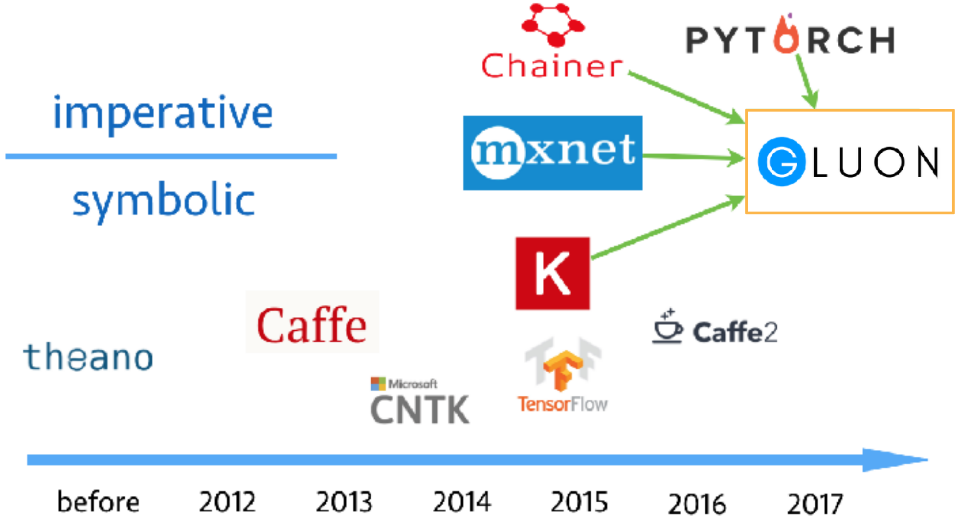
\includegraphics[scale=0.35]{gluon_strategy.png}
       \\ \scriptsize{\\[5pt]The strategy behind GLUON(from \cite{gluon-tutorial})\\}
     \end{frame}

     \begin{frame}
       \frametitle{Brief Reviews - 6/6}
       %% \begin{block}{} % alertblock {Deep Learning...}
       %%   \small{Deep Learning is an approach to AI that can safely be regarded as the study of models that involve a great amount of \textbf{composition of learned functions}\cite[p.8]{goodfellow}}
       %% \end{block}
       %% \vspace{0mm}

       \begin{columns}
         \column{0.5\linewidth}
         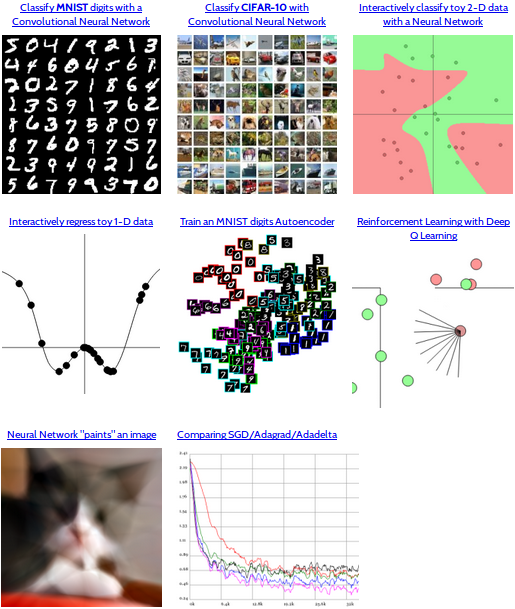
\includegraphics[scale=0.33]{convnetjs_demos.png}
         \column{0.49\linewidth}
         \centering
       
\includegraphics[scale=0.23]{logo_convnetjs.png}

         \begin{itemize}[<.->]
         \item \small{In-browser (or NodeJS server), single-file library by A. Karpathy}
         \item \small{Sequential (Keras-alike) building, saving trained models as JSON}
         \item \small{Low model coverage (no RNNs), but sufficient for many tasks}
         \item \small{Low performance, suitable for moderate inference or on-line learning}
         \item \small{Emphasis on interactivity (webapps) and communication (D3) of models}
         \end{itemize}
       \end{columns}
       \tiny{\\Browser Demos: CNN classification (MNIST and CIFAR), NN classification and regression, Autoencoder, reinf. learning with Deep Q Learning, color-regression (FCN) and comparing SGD/Adagrad/Adadelta (from \cite{convnetjs-web}).}
       %% \begin{center}
       %%   \\\scriptsize{From \cite[220]{goodfellow}: The computational graph corresponding to the following function composition:\\
       %%     $J = \mathcal{L}(y,  relu(x^TW^{(1)})^TW^{(2)}) + \lambda \sum_{w_i \in(W^{(1)}, W^{(2)})} {w_i^2} $ } 
       %% \end{center}
       
     \end{frame}
          
     \subsection{POPLAR} %%%%%%%%%%%%%%%%%%%%%%%%%%%%%%%%%%%%%%%%%%%%%%%%%%%%%%%%
     \begin{frame}[c] % [plain, c]
       \begin{center}
         \vspace{8mm}
         
\includegraphics[scale=0.18]{logo_poplar.png}
       \end{center}
     \end{frame}

        \begin{frame}
       \frametitle{The IPU}
       \vspace{-6mm}
        \begin{center}
          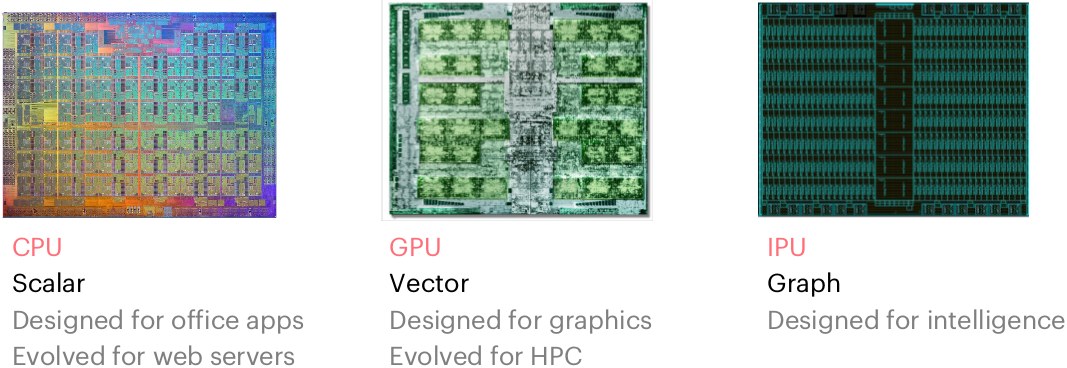
\includegraphics[scale=0.32]{cpu_gpu_ipu.png}
          \scriptsize{\\Intelligence requires a new architecture (from \cite{ipu-nips}).}
        \end{center}
        \begin{itemize}
        \item More bandwidth and memory for the models due to graph-based architecture
        \item Built-in suppor for algebra, low precision, noise generators, address-less communication
        \item Performance 2-3 orders of magnitude higher than best NVIDIA GPUs\cite{ipu-benchmarks}
       \end{itemize}
     \end{frame}

     \begin{frame}
       \frametitle{Poplar: Overview}
       From \cite{poplar-overview}, \cite{poplar-nips}:
       \begin{itemize}
       \item Dependencies: IPU drivers, C++11 library with \textit{poputil}, \textit{popops}, \textit{poplin}, \textit{poprandom}, \textit{popnn} (future: fft, robotics)
       \item Developed by GraphCore, library claimed to be OSS, but no public repos to the present date. Has Python API
       \item Deploys to IPU, like TF and MXNet (future: PyTorch, Caffe2, CNTK), but more optimized for it
       \item Translates into ``codelets'' that generate more vertices than TF graphs, usually millions (beyond tensor-centric)
       \item Deploys to IPU, like TF and MXNet, but more optimized for it
       \item Emphasis in non-dev tools for debugging and analysis
       \end{itemize}
     \end{frame}


     

     
     \subsection{Michelangelo} %%%%%%%%%%%%%%%%%%%%%%%%%%%%%%%%%%%%%%%%%%%%%%%%%%%%%%%%
     \begin{frame}[c] % [plain, c]
       \begin{center}
         \vspace{8mm}
         
\includegraphics[scale=0.1]{logo_uber.png}
       \end{center}
     \end{frame}

     
     \begin{frame}
       \frametitle{Michelangelo: Overview - 1/5}
       Like PyRo, developed by Uber. At the moment info only in \cite{michelangelo}.
       \begin{block}{} % alertblock {Deep Learning...}
         \small{Michelangelo allows \textbf{standardizing the workflows and tools} across teams through an end-to-end system that enables users across the company to easily \textbf{build and operate machine learning systems at scale.}}
       \end{block}
       \begin{center}
          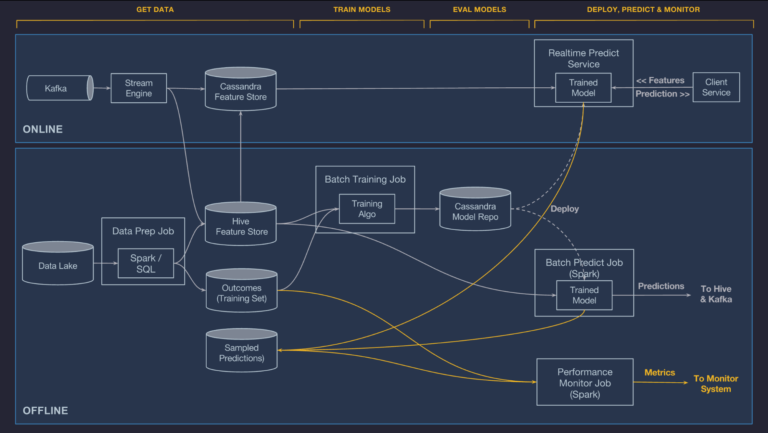
\includegraphics[scale=0.295]{michelangelo_pipeline.png}
          \scriptsize{\\Every workflow involving Michelangelo covers 6 steps: \textbf{manage data} (1), \textbf{train} (2) \textbf{evaluate} (3) and \textbf{deploy} (4) models,  \textbf{make} (5) and \textbf{monitor} (6) predictions.}
        \end{center}
     \end{frame}
     

        \begin{frame}
       \frametitle{Michelangelo: Overview - 2/5}
       \begin{enumerate}
       \item \normalsize{\textbf{Manage data}: Scalable, performant access to the company's data lake and ``feature store''. Online and offline, aided by a DSL subset of Scala}
       \item \normalsize{\textbf{Train models}: Encapsulated models running on Apache infrastructures. Supports different models including DNNs, time-series, k-means... and is extendible}
       \item \normalsize{\textbf{Evaluate models}: After training, a ``version object'' is stored with metadata and trained parameters, and can be easily inspected via an integrated, model-specific web UI (picture in next slide)}
       \item \normalsize{\textbf{Deploy models}: Offline, Online or as Library. Re-training and re-deployment can be automatically scheduled}
       \item \normalsize{\textbf{Make predictions}: Highest traffic models around 250000preds/s. }
       \item \normalsize{\textbf{Monitor predictions}: A percentage of the predictions can be used to generate on-going metrics, which can trigger accions when a given threshold is reached}
       \end{enumerate}
     \end{frame}


        \begin{frame}
          \frametitle{Michelangelo: Overview - 3/5}
          \begin{center}
            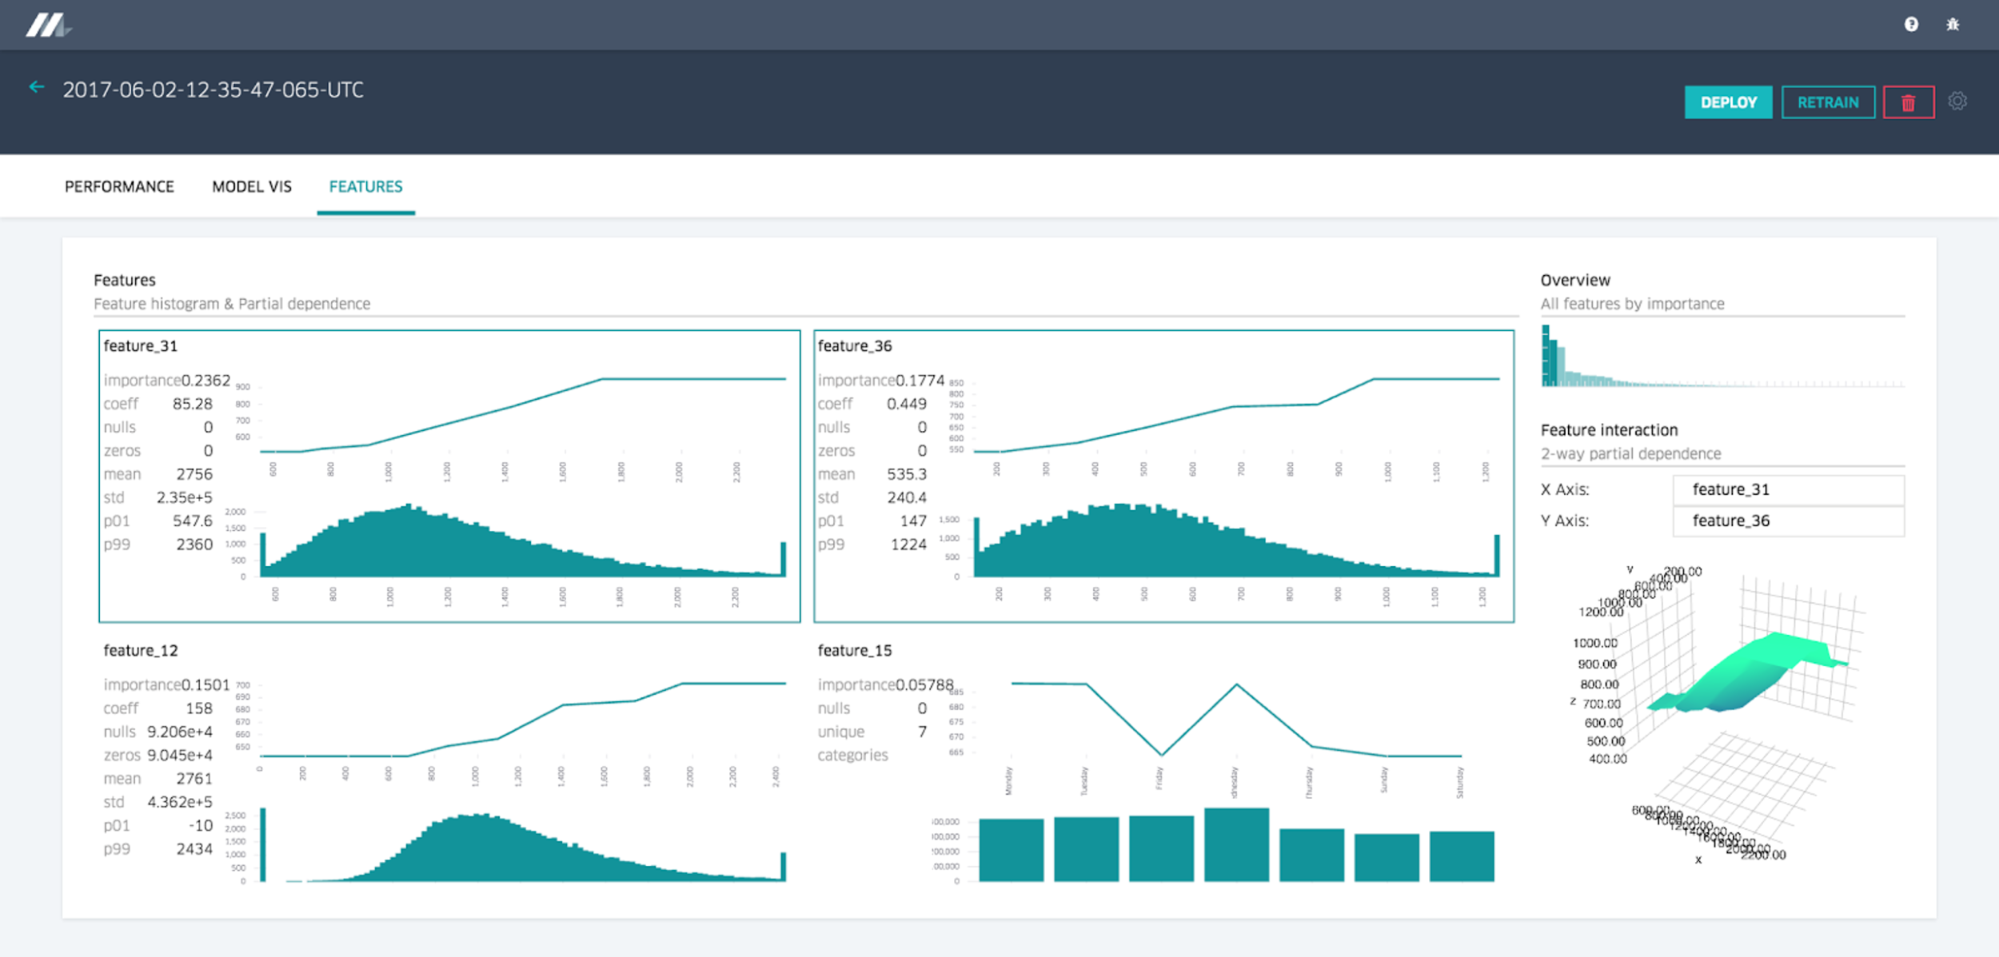
\includegraphics[scale=0.17]{michelangelo_overview.png}
            \scriptsize{\\Screenshot of Michelangelo's web UI for model evaluation\cite{michelangelo}.}
          \end{center}
        \end{frame}

        

        \begin{frame}
          \frametitle{Michelangelo: Overview - 4/5}
          
          \begin{columns}
            \column{0.5\linewidth}
            \begin{block}{} % alertblock {Deep Learning...}
              \small{Uber began development in 2015. Unlike other well-known Uber products like Horovod (distributed DL framework) and PyRo (PPL), \textbf{it hasn't been open sourced}, but it uses HDFS, Spark, Samza (Kafka+Hadoop), Cassandra (DB), MLLib, XGBoost, and TensorFlow.} % \\[15pt]
       \end{block}

         \column{0.49\linewidth}
         \centering
         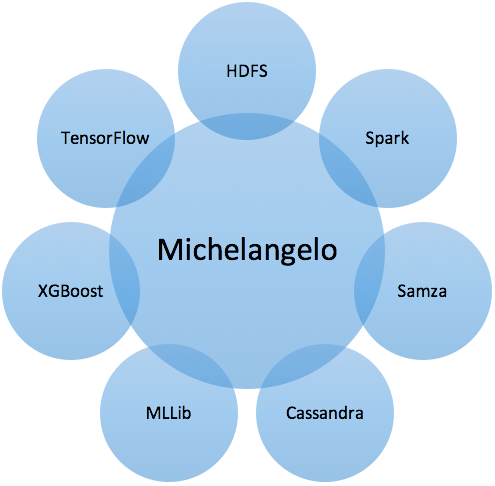
\includegraphics[scale=0.28]{michelangelo_oss.png}
       \end{columns}


          Challenges/Future:
          \begin{itemize}
          \item \small{\textbf{AutoML}: Integrated metalearning, model search}
          \item \small{\textbf{Model Visualization}: Currently good support for tree-based models only}
          \item \small{\textbf{Online Learning}: Add further functionality to the existing one}
          \item \small{\textbf{Distributed DL}: ``The user workflow of defining and iterating on deep learning models is sufficiently different from the standard workflow such that it needs unique platform support''}
          \end{itemize}
      
        \end{frame}

        \begin{frame}
          \frametitle{Michelangelo: Overview - 5/5}
          \begin{center}
            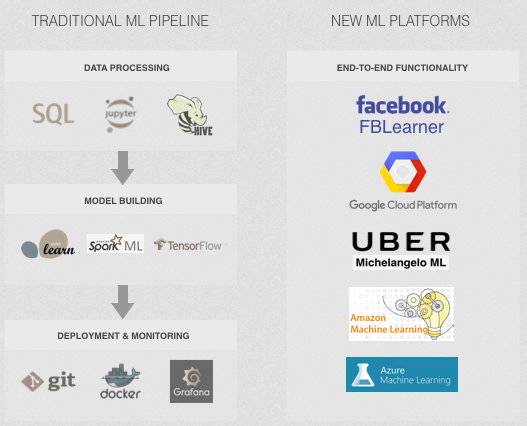
\includegraphics[scale=0.43]{evolution_ml_engineering.png}
            \scriptsize{\\``Large tech companies have recently started to use their own centralized platforms for machine learning engineering, which more cleanly tie together the previously scattered workflows of data scientists and engineers''\cite{evolution-ml}.}
          \end{center}
        \end{frame}

           
     %% \subsection{AML} %%%%%%%%%%%%%%%%%%%%%%%%%%%%%%%%%%%%%%%%%%%%%%%%%%%%%%%%
     %% \begin{frame}[c] % [plain, c]
     %%   \begin{center}
     %%     \vspace{8mm}
     %%     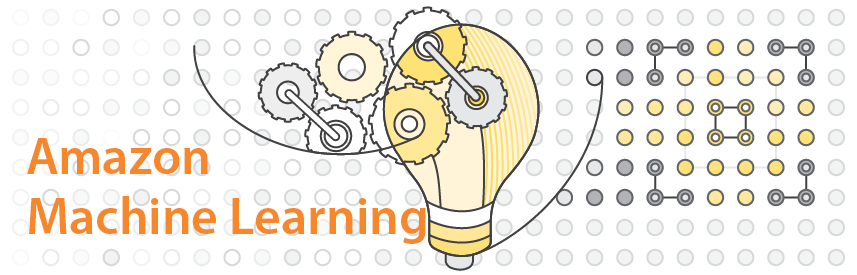
\includegraphics[scale=0.22]{logo_aml.png}
     %%   \end{center}
     %% \end{frame}

     
     %% \begin{frame}
     %%   \frametitle{Amazon Machine Learning: Overview}
     %%   Test
     %% \end{frame}


     %%%%%%%%%%%%%%%%%%%%%%%%%%%%%%%%%%%%%%%%%%%%%%%%%%%%%%%%%%%%%%%%%%%%%%%%%%%%%%%%%%%%%%%%
     \section{Sum-Up}
     \frame{\sectionpage}
     %%%%%%%%%%%%%%%%%%%%%%%%%%%%%%%%%%%%%%%%%%%%%%%%%%%%%%%%%%%%%%%%%%%%%%%%%%%%%%%%%%%%%%%%

     \begin{frame}
       \frametitle{Interaction among Frameworks}
       Many vectors of interaction:
       \begin{itemize}[<.->]
       \item \normalsize{Higher-order frameworks (e.g. Keras, Gluon)}
       \item \normalsize{Cross-platform serialization: from scripts (caffe to caffe2 \cite{caffe-to-caffe2}) evolved to specifications (ONNX\cite{onnx-v1})}
       \item \normalsize{Centralized platforms (e.g. Michelangelo, AML)}
       \item \normalsize{Common languages (most frameworks have a Python API)}
       \end{itemize}
       \vspace{5mm}
       Different strategies:
       \begin{itemize}[<.->]
       \item \normalsize{Easy performance of mainstream models/HW (f.e. Caffe2)}
       \item \normalsize{Popularity: broad coverage of platforms/languages (f.e. TF, CNTK)}
       \item \normalsize{Integration into specific environments (f.e. DL4J, ConvNetJS)}
       \item \normalsize{Emphasis on dynamic models (f.e. PyTorch, Chainer, DyNet)}
       \end{itemize}
     \end{frame}

%%      \begin{frame}
%%        \frametitle{Comparison among Frameworks}
%%        \begin{columns}% [t]
%%            \column{0.8\linewidth}
%%            % \hspace{-30mm}
%%            \centering
%%          \begin{tikzpicture}
%%            \tkzKiviatDiagram[scale=0.27,
%%              label space=9.2cm,
%%              radial  = 0,
%%              space=1,
%%              gap     = 1.05,
%%              lattice = 6]{
%%              \tiny{\textcolor{visiblered}{$\quad$1.platform/HW/\\[-6]$\quad$parall. support}},
%%              \tiny{\textcolor{visiblered}{\\[-1]2.run/train speed}},
%%              \tiny{\textcolor{visiblegreen}{\\[5]3.layer API}},
%%              \tiny{\textcolor{visiblegreen}{\\[5]4.model API}},
%%              \tiny{\textcolor{visiblegreen}{\\[-1]5.data tools}},
%%              \tiny{\textcolor{visiblegreen}{6.non-dev\\[-6]tools}},
%%              \tiny{\textcolor{visibleblue}{\\[5]7.documentation/\\[-6]learning curve}},
%%              \tiny{\textcolor{visibleblue}{\\[-8]8.Platforms/Languages/$\qquad\;$\\[-6] IDEs integration$\quad$}},
%%              \tiny{\textcolor{visibleblue}{\\[-8]$\qquad\qquad$9.HW/Parallelism\\[-6]$\qquad\qquad$transparency}},
%%              \tiny{\textcolor{visibleblue}{\\[2]10.healthy community/\\[-6] maintainability}}
%%            }
%%            \tkzKiviatLine[thick, % ultra thick
%%              color=green,
%%              % mark=none, % ball, mark size=5pt
%%              fill=green!10,
%%              opacity=1](4,5,5,3,6,2,4,5,4,4)
%%            \tkzKiviatLine[thick,
%%              color=blue,
%%              % fill=blue!10,
%%              opacity=0](4,3,5,3,3,6,4,3,3,5)
%%            \tkzKiviatLine[thick,
%%              color=red,
%%              % fill=red!10,
%%              opacity=0.5](4,5,5,5,4,6,4,3,2,3)

%%            % \tkzKiviatGrad[unity=1](1)
%%          \end{tikzpicture}
         
         
%%          \column{0.4\linewidth}
%%   \begin{tikzpicture}
%%            \tkzKiviatDiagram[scale=0.27,
%%              label space=9.5cm,
%%              radial  = 0,
%%              space=1,
%%              gap     = 1.05,
%%              lattice = 6]{
%%              \tiny{\textcolor{visiblered}{$\quad$1.platform/HW/\\[-6]$\quad$parall. support}},
%%              \tiny{\textcolor{visiblered}{\\[-1]2.run/train speed}},
%%              \tiny{\textcolor{visiblegreen}{\\[5]3.layer API}},
%%              \tiny{\textcolor{visiblegreen}{\\[5]4.model API}},
%%              \tiny{\textcolor{visiblegreen}{\\[-1]5.data tools}},
%%              \tiny{\textcolor{visiblegreen}{6.non-dev\\[-6]tools}},
%%              \tiny{\textcolor{visibleblue}{\\[5]7.documentation/\\[-6]learning curve}},
%%              \tiny{\textcolor{visibleblue}{\\[-8]8.Platforms/Languages/$\qquad\;$\\[-6] IDEs integration$\quad$}},
%%              \tiny{\textcolor{visibleblue}{\\[-8]$\qquad\qquad$9.HW/Parallelism\\[-6]$\qquad\qquad$transparency}},
%%              \tiny{\textcolor{visibleblue}{\\[2]10.healthy community/\\[-6] maintainability}}
%%            }
%%            \tkzKiviatLine[thick, % ultra thick
%%              color=green,
%%              % mark=none, % ball, mark size=5pt
%%              fill=green!10,
%%              opacity=1](4,5,5,3,6,2,4,5,4,4)
%%            \tkzKiviatLine[thick,
%%              color=blue,
%%              % fill=blue!10,
%%              opacity=0](4,3,5,3,3,6,4,3,3,5)
%%            \tkzKiviatLine[thick,
%%              color=red,
%%              % fill=red!10,
%%              opacity=0.5](4,5,5,5,4,6,4,3,2,3)

%% % \tkzKiviatGrad[unity=1](1)  
%%          \end{tikzpicture}

%%   \column{0.4\linewidth}
%%   hello

%%        \end{columns}
%%      \end{frame}



          
     \begin{frame}
       \frametitle{Kiviat Summary}
       \begin{columns}
         \column{0.5\linewidth} \centering \textbf{\textcolor{orange!80}{TF}/\textcolor{blue!60}{MXNet}/\textcolor{green!60}{CNTK}}
         \column{0.5\linewidth} \centering \textbf{\textcolor{violet!50}{PyTorch}/\textcolor{grey!80}{Caffe2}/\textcolor{visibleblue!70}{DL4J}}
       \end{columns}

       \begin{columns}
         \column{0.4\linewidth}
 \begin{tikzpicture}
           \tkzKiviatDiagram[scale=0.27,
             label space=7.7cm,
             radial  = 0,
             space=1,
             gap     = 1.05,
             lattice = 6]{
             \tiny{\textcolor{visiblered}{$\quad$1.}},
             \tiny{\textcolor{visiblered}{2.}},
             \tiny{\textcolor{visiblegreen}{3.}},
             \tiny{\textcolor{visiblegreen}{4.}},
             \tiny{\textcolor{visiblegreen}{5.}},
             \tiny{\textcolor{visiblegreen}{6.}},
             \tiny{\textcolor{visibleblue}{7.}},
             \tiny{\textcolor{visibleblue}{8.}},
             \tiny{\textcolor{visibleblue}{9.}},
             \tiny{\textcolor{visibleblue}{10.}}
           }
           % TENSORFLOW
           \tkzKiviatLine[ultra thick, % ultra thick
             color=orange!80,
             % mark=none, % ball, mark size=5pt
             fill=orange!30,
             opacity=1](6,3,5,5,5,4,5,5,5,5)
           % MXNET
           \tkzKiviatLine[ultra thick, % ultra thick
             color=blue!60,test,
             % mark=none, % ball, mark size=5pt
             % fill=blue!30,test
             opacity=1](6,5, 5,5,5,4, 5,6,5,5)
           % CNTK
           \tkzKiviatLine[ultra thick, % ultra thick
             color=green!60,
             % mark=none, % ball, mark size=5pt
             % fill=green!30,
             opacity=1](5,5,5,5,4,5,5,6,5,3)


           \end{tikzpicture}

         \column{0.6\linewidth}
 \begin{tikzpicture}
           \tkzKiviatDiagram[scale=0.27,
             label space=9.5cm,
             radial  = 0,
             space=1,
             gap     = 1.05,
             lattice = 6]{
             \tiny{\textcolor{visiblered}{$\quad$1.platform/HW/\\[-6]$\quad$parall. support}},
             \tiny{\textcolor{visiblered}{\\[-1]2.run/train speed}},
             \tiny{\textcolor{visiblegreen}{\\[5]3.layer API}},
             \tiny{\textcolor{visiblegreen}{\\[5]4.model API}},
             \tiny{\textcolor{visiblegreen}{\\[-1]5.data tools}},
             \tiny{\textcolor{visiblegreen}{6.non-dev\\[-6]tools}},
             \tiny{\textcolor{visibleblue}{\\[5]7.documentation/\\[-6]learning curve}},
             \tiny{\textcolor{visibleblue}{\\[-8]8.Platforms/Languages/$\qquad\;$\\[-6] IDEs integration$\quad$}},
             \tiny{\textcolor{visibleblue}{\\[-8]$\qquad\qquad$9.HW/Parallelism\\[-6]$\qquad\qquad$transparency}},
             \tiny{\textcolor{visibleblue}{\\[2]10.healthy community/\\[-6] maintainability}}
           }
           % PYTORCH
           \tkzKiviatLine[ultra thick, % ultra thick
             color=violet!50,
             % mark=none, % ball, mark size=5pt
             % fill=violet!20,
             opacity=1](4,4,6,6,5,4,5,5,5,5)
           % CAFFE2
           \tkzKiviatLine[ultra thick, % ultra thick
             color=grey!80,
             % mark=none, % ball, mark size=5pt
             fill=grey!17,
             opacity=1](5,6,5,4,5,3,3,5,5,5)
           % DL4J
           \tkzKiviatLine[ultra thick, % ultra thick
             color=visibleblue!70,
             % mark=none, % ball, mark size=5pt
             % fill=visibleblue!70,
             opacity=1](5,5,4,4,6,5,5,5,5,5)
         \end{tikzpicture}

         %% \\\scriptsize{second legend}
       \end{columns}
     \end{frame}





     %% %%%%%%%%%%%%%%%%%%%%%%%%%%%%%%%%%%%%%%%%%%%%%%%%%%%%%%%%%%%%%%%%%%%%%%%%%%%%%%%%%%%%%%%%
     %% \section{Discussion}
     %% \frame{\sectionpage}
     %% %%%%%%%%%%%%%%%%%%%%%%%%%%%%%%%%%%%%%%%%%%%%%%%%%%%%%%%%%%%%%%%%%%%%%%%%%%%%%%%%%%%%%%%%

     %% \begin{frame}
     %%   \frametitle{Conclusions and Follow-up}
     %%   \begin{itemize}
     %%   \item \Large Conclusions:
     %%     \begin{enumerate}
     %%     \item The chosen time/frequency representations are probably too sparse to allow any kind of regularization to be effective
     %%     \item basic preprocessing like cutting off non-melodic segments would have been instrumental
     %%     \item Histograms of the network weights would have helped the diagnose
     %%     \end{enumerate}
     %%     \vspace{5mm}
     %%   \item \Large Follow-up:
     %%     \begin{enumerate}
     %%     \item Train similar networks on the TDMS to confirm data issue
     %%     \item Incorporating the TDMS to other problem domains (f.e. western MGR)
     %%     \item Implementing the auralization ... sort of deconvolution for audio) as a diagnose tool to get a beter insight on the networks' problems
     %%     \end{enumerate}
     %%   \end{itemize}
     %% \end{frame}

     \setbeamercolor{background canvas}{bg=palette primary}
     \begin{frame}
       \frametitle{\centerline{\textbf{THANK YOU! Questions?}}}
       \begin{itemize}[<.->]

       \item  \textbf{Open-Source(d)}:
         \begin{itemize}[<.->]
         \item PyTorch (Facebook) $\leftarrow$ \textcolor{visiblered}{Torch (several)}
         \item Caffe2 (Facebook) $\leftarrow$ \textcolor{visiblered}{Caffe (BVLC)}
         \item TensorFlow (Google) $\leftarrow$ \textcolor{visiblered}{Theano (U. Montreal)}
         \item \small{MXNet (Apache)}
         \item \small{DL4J (Eclipse)}
         \item \small{CNTK (Microsoft)}
         \item \small{\textcolor{visiblered}{DyNet (Carnegie Mellon U.)}}
         \item \small{\textcolor{visiblered}{Chainer (U. Tokyo)}}
         \item \small{\textcolor{visiblered}{ConvNetJS (Karpathy)}}
         \item \small{POPLAR (GraphCore)}
         \item \small{And more (not covered): DIGITS (NVIDIA), Paddle (Baidu), Scikit-learn, SINGA and MLlib (Apache), neon (Intel)}
         \end{itemize}
       \end{itemize}
       \vspace{-2mm}

       \begin{minipage}[t]{0.45\textwidth}
         \vspace{0pt}
         \begin{itemize}[<.->]
           \item  \textbf{Closed-Source}:
             \begin{itemize}[<.->]
             \item \small{\textcolor{visiblered}{Mathematica (Wolfram)}}
             % \item \small{AML (Amazon)}
             \item \small{Michelangelo(Uber)}
             \end{itemize}
           \end{itemize}


       \end{minipage}%
       \hfill
       \begin{minipage}[t]{0.55\textwidth}
         \vspace{0pt}
         \begin{itemize}[<.->]
           \item  \textbf{Higher-Order}:
             \begin{itemize}[<.->]
             \item \small{\textcolor{visiblered}{Keras (on TF, Theano or CNTK)}}
             \item \small{\textcolor{visiblered}{Skorch (wraps PyTorch)}}
             \item \small{\textcolor{visiblered}{GLUON (on MXNET, CNTK)}}
             \end{itemize}
           \end{itemize}
       \end{minipage}
     \end{frame}

     %%%%%%%%%%%%%%%%%%%%%%%%%%%%%%%%%%%%%%%%%%%%%%%%%%%%%%%%%%%%%%%%%%%%%%%%%%%%%%%%%%%%%%%%
     % \appendix
     \section{References}
     % \frame{\sectionpage}
     %%%%%%%%%%%%%%%%%%%%%%%%%%%%%%%%%%%%%%%%%%%%%%%%%%%%%%%%%%%%%%%%%%%%%%%%%%%%%%%%%%%%%%%%

     \begin{frame}[c] % [plain, c]
       \begin{center}
         \vspace{8mm}
         \LARGE References
       \end{center}
     \end{frame}

     
     \begin{frame}[allowframebreaks]
       \bibliographystyle{apalike}
       \tiny \printbibliography
     \end{frame}

\end{document}

















